\chapter{Introduction}
\sloppy
\gls{tm} biology is a huge and varied field that is ultimately the study of the interface between compartments of the cell.
\gls{tmp}s include some of the most critical to life proteins as well as a large number of drug targets.
However, the experimental inaccessibility of the \gls{tmh} has hampered the progress of study compared to their globular structural analogues.
Despite progress over the last decade, the understanding of the relationship between the sequence and function of a \gls{tmh} is incomplete.

In this chapter we will place the \gls{tmh} problem in context, then describe the important biological aspects of the \gls{tmh}, and discuss tools and methods that allow us to analyse and describe the nuanced differences between these \gls{tmh} sequences.

\section{Transmembrane proteins}

\subsection{A brief history of the discovery and exploration of the transmembrane proteins}

Due to the ability to segregate biochemical environments, the cellular barrier has been described as one of the fundamental pillars of life as we know it~\cite{Ladokhin2015}.
The significance of the cellular barrier was first noted in 1665 with the dawn of the microscope when Robert Hooke described the cell wall of the cork plant (Figure \ref{fig:history}A), with the clear distinction of the barrier giving rise to the term ``cell'' \cite{Donaldson2010, hooke1961micrographia}.

%Some waffle about Hooke, Schwan, and Virchow

\begin{figure}[ht!]
\centering
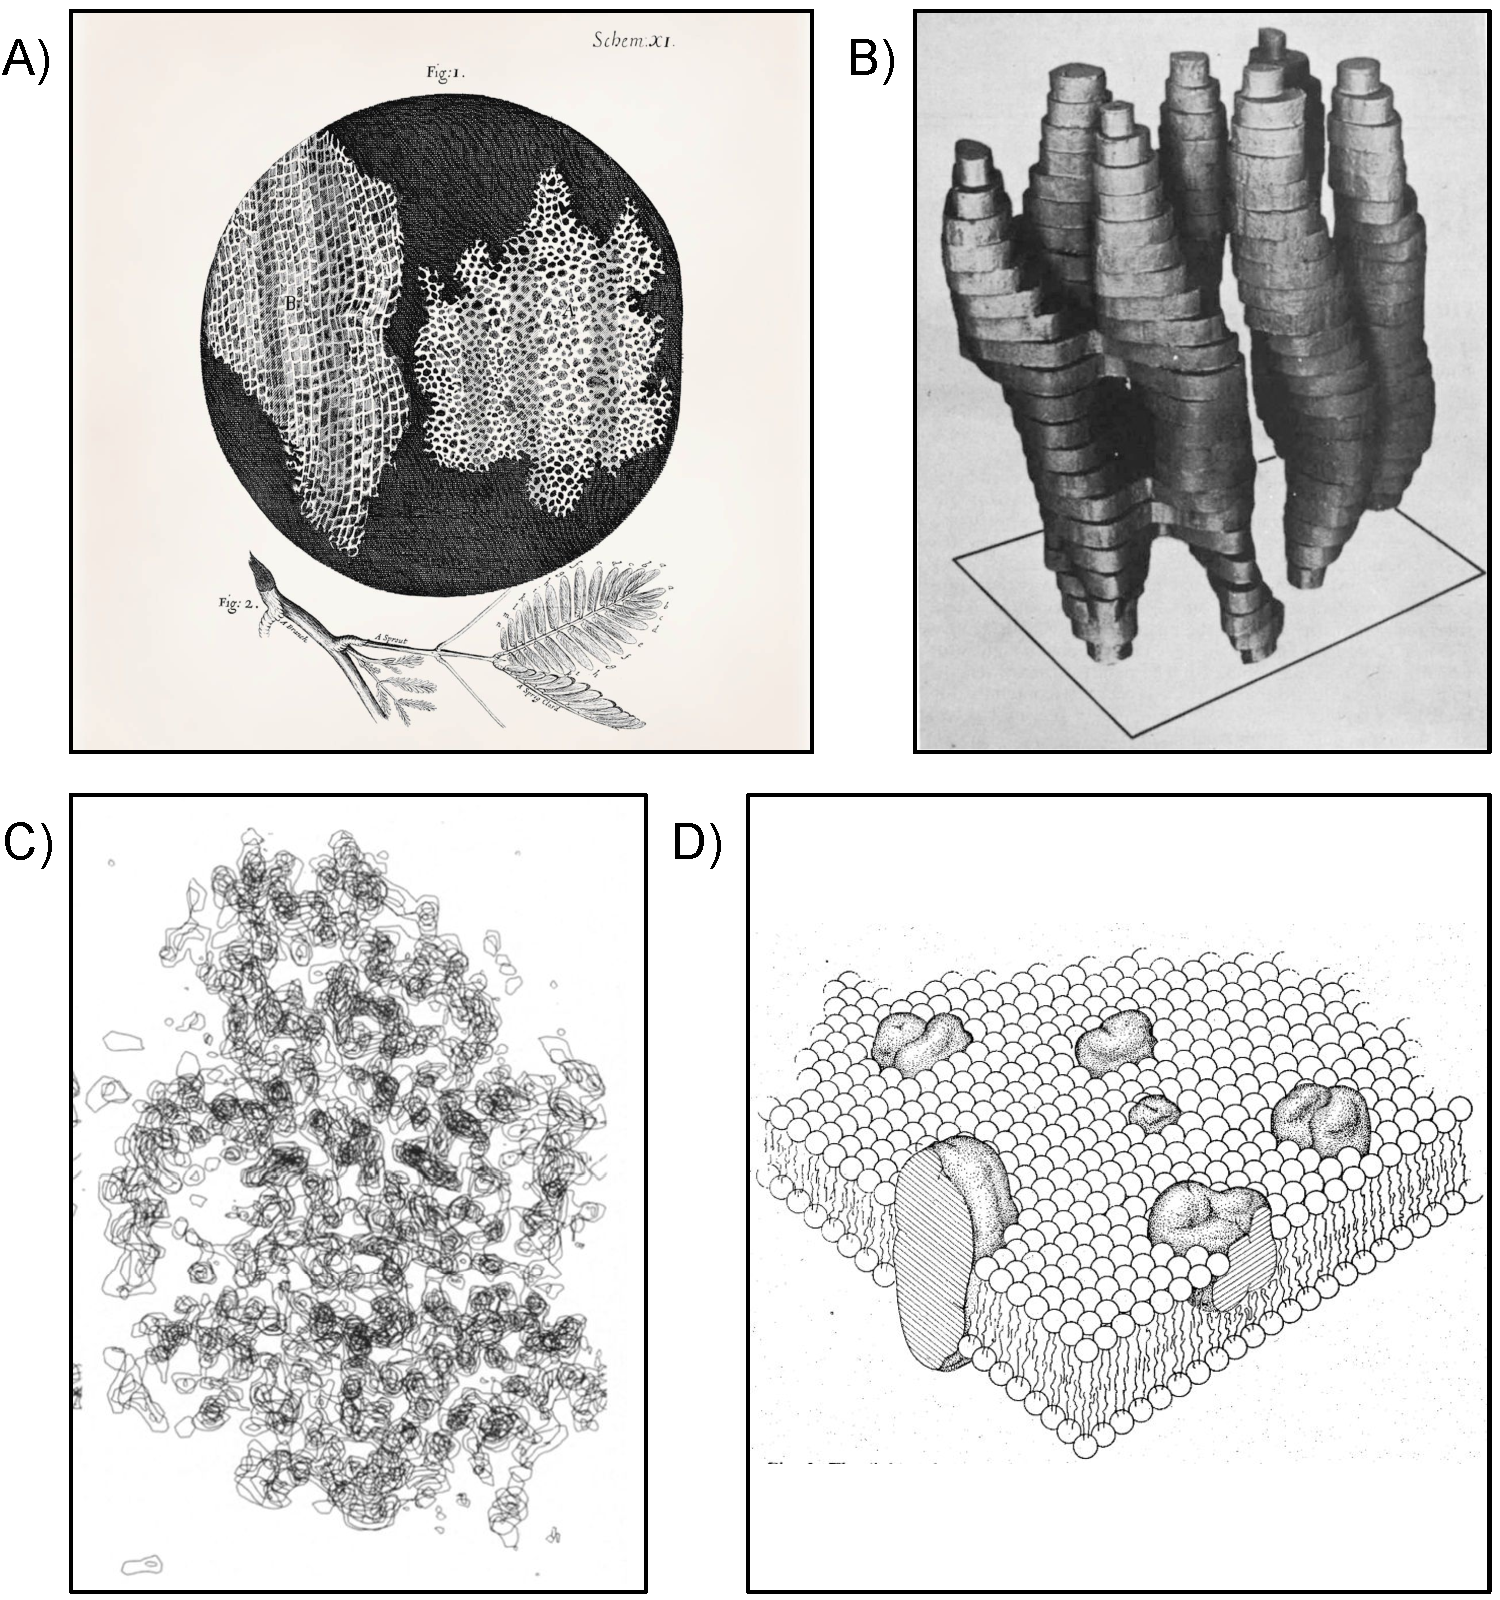
\includegraphics[width=1\textwidth]{Intro/history}
		\captionof{figure}[A selection of figures demonstrating important discoveries of membrane proteins and their environment.]{\textbf{A selection of figures demonstrating important discoveries of membrane proteins and their environment.}
		A) (Above/``Fig 1'') A diagram of the cork plant as viewed through an optical microscope drawn by Hooke circa 1665.
		Note the observable cellular barrier between what we now know to be the plant cells.
		(Below/``Fig 2'') The cork plant used in the microscope observations.
		From Hooke, republished in 1961 \cite{hooke1961micrographia}.
		B) The first near\--atomic resolution (7\angstrom~resolution map) structure of a \gls{tmp} acquired by \gls{em}.
		This is a model of the 7\gls{tm} bacteriorhodopsin single protein from the purple membrane viewed roughly parallel to the plane of the membrane.
		From Henderson \& Unwin, 1975 \cite{Henderson1975}.
		C) The electron density map of the first crystal structure of a \gls{tmp} \cite{Deisenhofer1984}.
		The image shows 11 layers with contours representing 1.2\angstrom~between layers at 3\angstrom~resolution.
		As in B, this structure is from phototrophic purple bacteria.
		The chromophores are made up of cytochrome (can be seen at the top of the image) and the H\--subunit (which can be seen at the bottom).
		From Deisenhofer \textit{et al.,} 1984.
		D) The first drawing in which the fluid mosaic model was presented in the bilayer.
		From Singer \& Nicolson, 1972 \cite{Singer1972}
		}

\label{fig:history}
\end{figure}

Throughout the early 20th century several theories were explored regarding the composition of the membrane.
In 1925, by scrutinising the concentration of chromocytes in the blood, and the surface area of the cells from blood from a variety of mammals Gorter and Grendel concluded that: ``chromocytes are covered by a layer of fatty substances that is two molecules thick'' \cite{Gorter1925}.
This established the awareness of the lipid bilayer.
Later, the popular Danielli and Davson model correctly identified a phospholipid bilayer, however also incorrectly suggested a lipoid space existed within the phospholipid bilayer \cite{Danielli1935}.
Eventually, as these ideas were explored, the fluid mosaic model was established in 1972 (Figure \ref{fig:history}D)\cite{Singer1972}; the membrane has a fluid behaviour, due to the gel\--like nature of its composition, which allows proteins to move throughout the membrane bilayer.

In order to fully understand the relationship between \gls{tmp}s and the membrane, molecular details would be needed.
By the 1970s, reasonably detailed structures of membrane\--spanning segments of \gls{tmp}s were available by \gls{em} \cite{Henderson1975} (Figure \ref{fig:history}B).
However, the real goal was to have the atomic resolution available.
The advent of x\--ray crystallography through the first half of the 20th century showed that it was possible to solve atomically resolved structures of small organic molecules \cite{Lonsdale1928, Dickinson1923} and larger proteins such as a steroid \cite{Carlisle1945}, penicillin \cite{Hodgekin1949}, and vitamin B12 \cite{HODGKIN1955}.
Dorothy Hodgekin was awarded the Nobel prize for chemistry in 1964 for the elucidation of these complex structures \cite{NobelMedia2018a}.
7 years after the creation of the \gls{pdb} \cite{Bernstein1978}, the first \gls{tmp} was successfully solved by x\--ray crystallography in 1984 \cite{Deisenhofer1984} (Figure \ref{fig:history}C).
Because of this discovery Johann Deisenhofer, Robert Huber, and Hartmut Michel won the Nobel prize in chemistry in 1988 for solving with atomistic resolution the 3D structure of a photosynthetic reaction centre \cite{NobelMedia2018}.
In the following decades, x\--ray crystallography of \gls{tmp}s, despite the challenges therein, remained the predominant method of generating the structure of \gls{tmp}s \cite{Carpenter2008}.
Currently, we are in a revolution of \gls{tmp} structural acquisition, which will be discussed further in section \ref{section:revolution}.

\subsection{Transmembrane proteins in disease}
Membrane\--bound proteins underpin almost every biological process directly, or indirectly, from photosynthesis to respiration.
Integral \gls{tmp}s are encoded by between a third to a half of the genes in the human genome~\cite{Hopkins2002, Almen2009, Wang2013} and account for 40\% of drug targets \cite{Overington2006} which reflects their biological and physiological importance.
\gls{tmp}s allow biochemical pathways that traverse the various biological membranes used in life, either by transporting molecules or transducing signals across the bilayer.
Misfolding of these proteins during the complex process of translocation is common in both normal and diseased cells and the mechanisms of folding are actively studied even recently revealing new systems of translocation, such as the role of the \gls{emc} in both co\--translational \cite{Shurtleff2018} and post\--translational \cite{Guna2018} \gls{tmp} integration.
Mutations tend to cluster in the \gls{tmh} regions of the genes \cite{Sanders2004}, which can cause the misfolding.
Glycine to arginine mutations occur statistically more frequently in \gls{tmh}s compared to their globular $\alpha$\--helix counterparts \cite{Partridge2002}.
This can result in a range of diseases including but not limited to cystic fibrosis caused by mutations in the cystic fibrosis conductance regulator \cite{Riordan1989}, Charcot\--Marie\---Tooth disease caused by mutations in the PMP22 gene \cite{Roa1993} and the connexin 32 gene \cite{Fairweather1994}, diabetes insipidus caused by mutations the aquaporin 2 water channel \cite{vanLieburg1994}, retinitis pigmentosa caused by a point mutation in rhodopsin \cite{Dryja1990}, and Niemann\--Pick disease that contains over 200 disease\--causing mutations identified \cite{Gelsthorpe2008, Park2003, Scott2004, Fernandez-Valero2005}.

\subsection{The transmembrane protein problem}

Studying \gls{tmp}s in a laboratory typically presents several challenges not so often faced when investigating their globular counterparts which are pointed out in a review by Seddon \textit{et al.,} 2004~\cite{Seddon2004}.
\gls{tmp}s are typically difficult to obtain in a useful quantity.
They do not exist in high enough quantities naturally, and overexpression often results in aggregation in the cytoplasm.
Also, the complexity of their native environments limits structural studies.
Even relatively simple lipid bilayers cannot be probed by conventional structural techniques, so study in the native state by traditional structural methods is difficult and involves suspending the protein in detergent or lipid environments, leading to difficulties in sample preparations.
Their insolubility in aqueous solutions also leads to the requirement of speciaised synthetic \textit{in vitro} systems to be used, which have been difficult to introduce purified proteins into \cite{Seddon2004}.

In addition to the practical difficulties in studying \gls{tmp}s, it has become clear that they have a rich structural diversity.
Throughout the 1990s the concept of a \gls{tmh} was simple and fairly assured: they were greasy peptides of around 30{\AA} in length, often bundled together and oriented perpendicularly to the membrane \cite{VonHeijne2006}.
By 2007, crystallography had elucidated 368 \gls{tmp} structures from 148 unique proteins \cite{Carpenter2008}.
Whilst this accumulation of structures was exponential, at the same time, there were in excess of 50,000 protein structures in the PDB.
What became clear when examining the newly avaiable large number of \gls{tmp}s was that although the classic \gls{tmh} structures were broadly prevalent, these structures contained a plethora of unusual \gls{tmh}s \cite{VonHeijne2006}.
\gls{tms}s are capable of partial spanning of the membrane, spanning using oblique angles, and even lying flat on the membrane surface~\cite{VonHeijne2006, Elofsson2007}; the classical model was incomplete.
Even recently, there is a contingency in the  \gls{tmp} biology field that despite progress over the last decade there is still a lack of information regarding the relationship between \gls{tmh} sequences and function, \gls{tmh} structure, intra-membrane \gls{tmp} assembly, and the behaviour of \gls{tmh}s in the lipid bilayer; the native biological environment of \gls{tmh}s~\cite{Ladokhin2015}.

Furthermore, the insertion and formation of the unusually orientated \gls{tmh}s and of the more traditional \gls{tmh}s have been shown to be underpinned by complex thermodynamic equilibrium and electrostatic interactions~\cite{Cymer2015, Elisa2012, Ismail2015}.
As well as being a biophysically convoluted system, \gls{tmh}s are biologically functional beyond anchoring in many cases.
\gls{tms}s have been identified as regulators of protein quality control and trafficking mechanisms, shifting the idea away from \gls{tmh}s broadly exclusively functioning as anchors~\cite{Hessa2011}, and crucially this function beyond anchoring can be revealed by sensitive analysis of the sequence information alone~\cite{Wong2011, Wong2012}.

There is also an issue of silent homology extension from $\alpha$\--helices \cite{Wong2010}.
\gls{tmh}s often share sequence composition similarities due to membrane requirements and restraints, not necessarily due to common ancestry which underpins homology\--based domain libraries like Pfam \cite{Finn2016} and SMART \cite{Letunic2012}.
It was found that between 2.1\% and 13.6\% of Pfam hits for \gls{sp}s or \gls{tms}s are positive hits that were misreported as homologous among distantly related proteins in Pfam \cite{Wong2010}.
%When predicting the function of any protein, one follows the dicta that function is facilitated by form, and form is determined by the sequence; the more similar the sequences, the more likely that the function is similar.
%For globular soluble proteins having the same folds induces strict biochemical restrictions on the packing of a hydrophobic protein core which requires similarity of non\--polar residue patterns.
%\cite{Wong2010}.
%In the case of \gls{sp}s or \gls{tms}s the physical constraints are similar for all \gls{tmp}s and so matching is indeed merely a reflection of the physical environment of the bilayer, not the common ancestry.
%it appears that between 2.1\% and 13.6\% of Pfam hits for \gls{sp}s or \gls{tms}s are indeed false positive results~\cite{Wong2010}.

\subsection{The transmembrane protein revolution}\label{section:revolution}
Over the last decade or so, several significant steps have been made toward overcoming the challenges in solving the structures of \gls{tmp}s.
Firstly, improvements in expression and purification occurred thanks to cleavable green fluorescent protein (allowing protein tracking during purification) \cite{Drew2005, Kawate2006} and antibody tagging for purification \cite{Eshaghi2005} at the colony level \cite{Cornvik2005} greatly increased the throughput of \gls{tmp} expression and purification.

\begin{figure}[ht!]
\centering
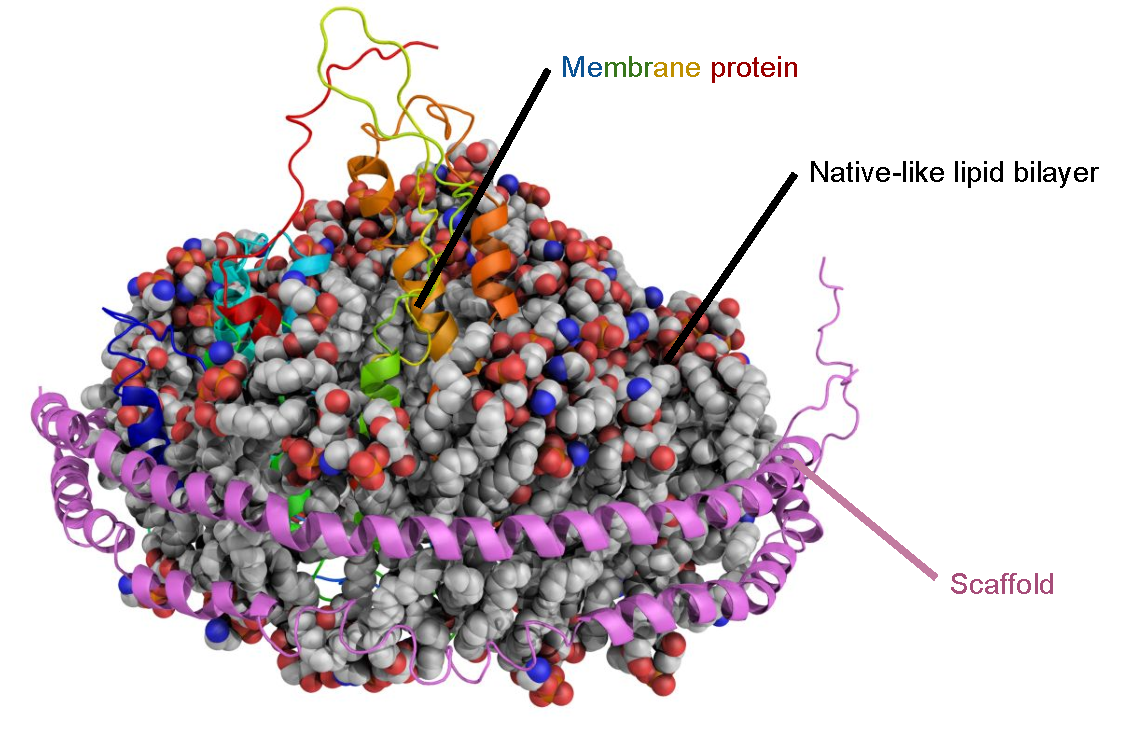
\includegraphics[width=1\textwidth]{Intro/revolution}
		\captionof{figure}[The structure of SecYE in a nanodisc at near atomic resolution.]{\textbf{The structure of SecYE in a nanodisc at near atomic resolution.}
		A single particle cryo\--\gls{em} structure of SecYE in complex with the ribosome (not shown) with the \gls{tmh}s held in a reconstituted nanodisc (PDB code 4v6m \cite{Frauenfeld2011}).
		The resolution is 7.1~\angstrom.
		The protein structure is depicted by a rainbow coloured cartoon in the centre of the assembly.
		The lipids are modelled as spherical atoms coloured by atom (carbon and hydrogen are white, oxygen is red and nitrogen is blue).
		The peptide scaffold is shown in pink.
		}

\label{fig:revolution}
\end{figure}

Since the folding of the \gls{tmp} often depends on the lipid environment and finding conditions that encourage protein stability was shown to improve crystallisation \cite{Carpenter2008, Rosenbusch2001}.
The technology behind nanodiscs was originally published in 2002 \cite{Bayburt2002}.
The structure of the nanodisc is formed from two scaffold peptide helices wrapped around a group of self\--associating phospholipids (Figure \ref{fig:revolution}A).
The method was originally shown to be a viable method for obtaining native condition \gls{tmp} crystals for cytochrome P450 \cite{Duan2004}.
Nanodiscs have been routinely used to much more easily obtain crystal structures.
Nanodiscs overcome some of the major challenges caused by the hydrophobic helices and a more faithful representation of the biological membranes than alternative model membranes like liposomes~\cite{Borch2009}.

Still, the challenge remained of getting crystals of sufficient quality for x\--ray diffraction.
Although many \gls{tmp}s readily formed low\--resolution 2D crystals for cryo\--\gls{em}~\cite{Vinothkumar2015, Raunser2009}, and genome sequencing resulted in an exponential increase in structures derived from x\--ray crystallography \cite{Vinothkumar2010}, the dependency on crystallising \gls{tmp}s has always resulted in a hindrance.

In a full circle from \gls{em} study of the fluid mosaic model in the 1970s \cite{Singer1972}, once more \gls{em} techniques were applied to \gls{tmp}s as single molecules (Figure \ref{fig:revolution}A).
This method escapes the need for \gls{tmp} crystals \cite{Vinothkumar2015} and the presence of the sub 3\angstrom~ structures \cite{Grant2015, Bartesaghi2015} utilising this method have exceeded the near atomistic resolutions that were called a revolution in \gls{tmp} biology, not a year earlier \cite{Kuhlbrandt2014}.


\subsection{The role of bioinformatics in transmembrane biology}

Due to the experimental difficulties of working with \gls{tmp}s, often it is only possible to experiment on the \gls{tmp}s \textit{in silico}, or at least common tasks that would involve expensive time\--consuming processes become trivialised, for example identifying \gls{tm} regions in a protein of known sequence.

Traditionally, the role of bioinformatics has been to predict \gls{tm} regions of a protein.
There are countless methods that can perform this.
Many rely on statistical patterns to identify \gls{tmh}s such as the neural network approach of MEMSAT3 \cite{Jones2007} Hidden Markov models used in TMHMM \cite{Krogh2001}, HMMTOP \cite{Tusnady2001}, S\--TMHMM \cite{Viklund2004}, OCTOPUS \cite{Viklund2008}, Phobius \cite{Kall2004}.
Unsatisfied with a statistical approach, Scampi seq \cite{Bernsel2008} uses a first principals method following the Kyte \& Doolittle suggestion 26 years previously that a biophysical scale can predict \gls{tmh}s \cite{Kyte1982} and applies a score based on the von Heijne biological scale \cite{Hessa2007}.

Predicting the presence of a typical \gls{tmh} based on a protein sequence is currently a fairly trivial task and typically relies on a consensus of several prediction programs, such as the automated TRANSMEM annotation used by UniProt \cite{TheUniProtConsortium2014}.
Yet several challenges remain in separating \gls{sp}s from \gls{tmh}s \cite{Petersen2011} and correctly predicting the topology of a \gls{tmp}.

Despite being able to identify \gls{tmh}s, our understanding of the specific biochemical role they play in the cell often requires intense study.
As more data is becoming available bioinformatic methods that use multiple biochemical traits in conjunction with hydrophobicity are starting to be able to understand if a \gls{tmh} has a functional role beyond anchoring \cite{Wong2011, Wong2012}, and the protein trafficking signals held within some \gls{tmh}s \cite{Guna2018}.

Despite the advances in the availability of \gls{tmp} structures over the last decade, most are obtained from membrane free environments via x\--ray diffraction of crystals, single\--molecule cryo\--\gls{em} and NMR \cite{Vinothkumar2015, Stansfeld2015}.
The relationship between the membrane and \gls{tmp}s is underpinned by complex thermodynamic and  electrostatic equilibrium \cite{Cymer2015}.
Once inserted the protein does not leave the membrane as a result of the \gls{tmh} being very hydrophobic.
This hydrophobicity of \gls{tmh}s and the hydrophobicity of the lipid tails means that they self\--associate and this association is entropically driven by water.
Another way of describing it is that they dissociate from the water.
The overall $\Delta G$ for a \gls{tmh} in the membrane is -12kcal${mol}^{\--1}$~\cite{Cymer2015}; the association of the helix in the membrane is typically spontaneous but complex owing to interactions with other \gls{tmh}s in the membrane as well as \gls{tmp}\--lipid interactions.
Although sometimes there are bound lipids and detergents included in the crystal lattice, or the \gls{tmp}s are integrated into a micelle or bicelle environment this is often insufficient to account for the complex lipodynamics of the membrane\--\gls{tmh} interactions \cite{Coskun2011, Stansfeld2015}.

\begin{figure}[ht!]
\centering
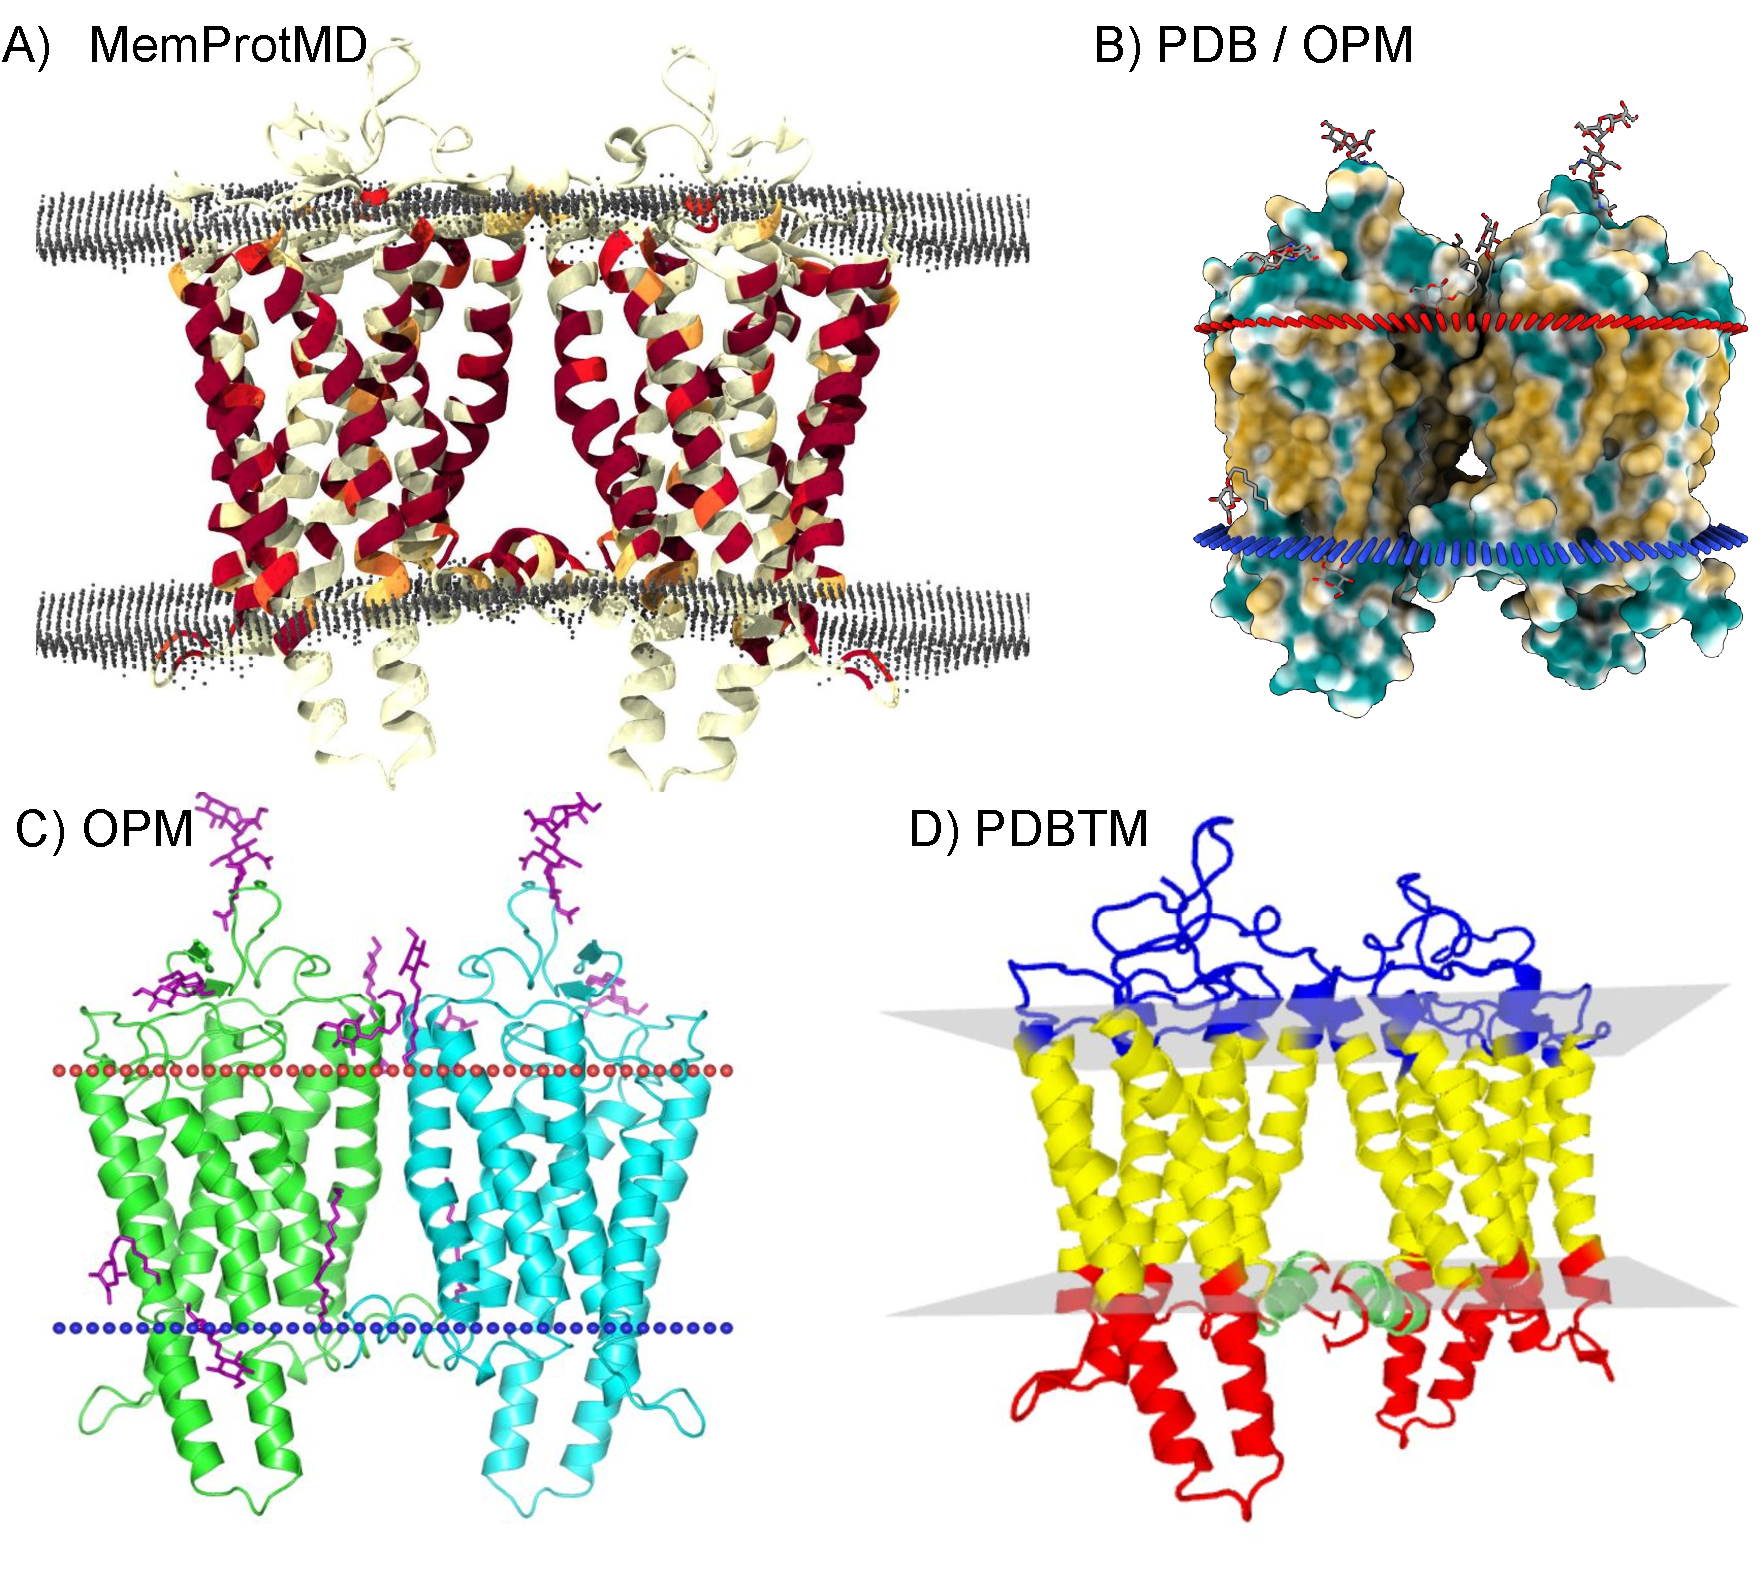
\includegraphics[width=1\textwidth]{Intro/3cap}
		\captionof{figure}[A comparison of a single structure held by commonly used structural transmembrane protein databases.]{\textbf{A comparison of the raw outputs from commonly used structural transmembrane protein databases.}
		The example used here is a ligand\--free \gls{gpcr} rhodopsin (\gls{pdb} 3cap)~\cite{Park2008}.
		A) The structure held by MemProtMD \cite{Stansfeld2015}. A cartoon of the structure coloured according to hydrophobicity. Red indicates hydrophobic residues and the cream colour represents hydrophilic residues. Note the flexing and distortion of the membrane.
		B) The RCSB PDB \cite{Berman2000} showing the hydrophobic patches on the surface (yellow is hydrophobic, cyan is hydrophilic) of the membrane proteins using OPM for topological orientation \cite{Lomize2012}.
		The blue lines indicate the cytoplasmic side whilst the red indicates the extracellular side.
		C) The cartoon structure of 3cap from OPM \cite{Lomize2012} coloured by the protein chain.
		Again, the blue lines indicate the cytoplasmic side whilst the red indicates the extracellular side.
		D) The PDBTM \cite{Kozma2012} record coloured by the \gls{tm} regions predicted by TMDET \cite{Tusnady2005} in yellow, intramembrane regions in green.
		In this case, the non\--membrane components are coloured according to side 1 and side 2 rather than a topological prediction.
		}

\label{fig:3cap}
\end{figure}

There have been several approaches used to attempt to find a more biologically relevant structure contextualised in the membrane (Figure \ref{fig:3cap}).
OPM \cite{Lomize2012} and PDBTM \cite{Kozma2012} use simplified models of the membrane's hydrophobic environment to orientate the \gls{tmp} into position.
MemProtMD \cite{Stansfeld2015} uses explicit lipids, a phosphatidylcholine bilayer, in a flexible \gls{md} simulation  along with \gls{tmp}s accessed from the PDB \cite{Berman2000}.
These approaches allow us to enhance our understanding of the \gls{tmp} structures in the context of the membrane environment.

\section{Biological membranes}
\subsection{Membrane lipids}
The compartmentalisation of cellular biochemistry is arguably one of the most significant events to have occurred in evolution and is certainly one of the fundamental prerequisites for life~\cite{Koshland2002}.
The proteins that allow life to use this biochemical barrier are perhaps equally important.
Together, the lipid bilayer and proteins therein allow complex biochemical systems that facilitate life as we know it.

It is critical to understand that the lipid bilayer and the transmembrane $\alpha$ helices are inextricably linked..
Often \gls{tmh}s reflect the membrane environments they exist in, for example, the hydrophobicity, asymmetry, and thickness of the membrane lipids are reflected when looking at large numbers of \gls{tmp}s~\cite{Sharpe2010}.

The lipid membranes influence the local structure, dynamics, and activity of proteins in the membrane in non-trivial ways~\cite{Bondar2010, Bondar2009, Jardon-Valadez2010, Kalvodova2005, Urban2005, White2001a, Jensen2004, Henin2014}, as well as protein folding~\cite{Kauko2010}.

%Add references about the hydrogen bonds (white2005 and another one...) %Perhaps this wedge of citations should be expanded.

The lipids that make up these membranes are very diverse, and not only do different cells have different membrane compositions but so do different subcellular compartments which again is reflected in the \gls{tmh} composition of \gls{tmp}s~\cite{Sharpe2010, VanMeer2008}.

They consist of a polar head group and a hydrophobic region and so are described as being amphiphilic molecules.
This factor, along with geometric constraints of the membrane lipids causes them to not only be insoluble molecules but also that they readily self-associate into complex ordered structures that have been demonstrated \textit{in silico} with coarse grain \gls{md} simulations~\cite{Scott2008}.
This self\--association is entropically driven by water molecules.
There is a rich variety of lipid molecules that make up the biological membranes.
Furthermore, the bilayer maximises van der Waals interactions between the closely-packed hydrocarbon chains, which contributes to the stability of the bilayer.
This can be seen even in relatively early \gls{md} simulations~\cite{Goetz1998}.

The majority of lipids in higher organism membranes are phospholipids, sphingolipids, and sterols.
The hydrophobicity of a membrane lipid can be caused by several features; (i) aliphatic chains such as in the most abundant membrane lipids, glycerophospholipids and the sphingolipids, (ii) aromatic groups, or (iii) polycyclic structures such as the sterols most abundantly of which in mammals is cholesterol ~\cite{Helenius1975, Lichtenberg1983}.
Phospholipids are composed of a glycerol molecule.
Bonded to the glycerol molecule are two hydrophobic fatty acid tail groups and a negatively-charged polar phosphate group.
The polar phosphate group is modified with an alcohol group.
Often these are represented as a polar head group with two fatty chains extending into the membrane, and a bilayer is formed from two sheets of these molecules with the polar headgroups facing outwards towards either side of the membrane and the fatty side chains filling the interior of the membrane space (Figure \ref{fig:history}D).

%At some point the membrane phases should be discussed.
%Similar to the diagram here perhaps: http://popups.ulg.ac.be/1780-4507/index.php?id=6568

It has been known for almost 4 decades that biological bi\--layer membranes are asymmetric~\cite{Singer1972, OpdenKamp1979}.
For example, in the outer membranes of Gram-negative bacteria, the outer membrane leaflet contains lipopolysaccharide, whilst the inner is a mixture of approximately 25 phospholipid types~\cite{VanMeer2008}.
Adding to the membrane asymmetry composition story, a thorough analysis of residue composition in yeast and human \gls{tmh} regions revealed intra-membrane leaflet composition asymmetry in the \gls{er}, but not the Golgi~\cite{Sharpe2010}.
Furthermore, protein-lipid interactions have been shown to be determinants of membrane curvature~\cite{Jensen2004}, and undertake complex orientations and conformations to allow for hydrophobic mismatch~\cite{Planque2003}.

%The evolutionary theories behind these various membrane compositions emerging are complex and remain in dispute.
%A popular theory is that eukaryotic cells used mitochondria as the ATP synthesisers to provide an energetic boost, the result of which was a massive shift in the evolution of novel eukaryotic protein folds, membrane\--bound organelle structures, sexual reproduction, and complex inter-cellular cooperation in the form of multicellular organisms~\cite{Lane2005, Lane2015}.
%A lot of this theory rested on the idea that mitochondrial membranes within the eukaryotic cells were energetically favourable, however, more recent experimentation disputes this claim~\cite{Lynch2017}.

\subsection{Membrane potential}
Simply put, membrane potential is the voltage across a membrane.
If the membrane is permeable to a certain type of ion, then the ion will experience an electrical pulling force during the diffusion process that pulls toward the ``preferred'' biological location.
This clearly depends on a chemical component involving both the charge and ion concentration gradient.
There are various ways of estimating the membrane potential \textit{ab initio}.

The Nernst equation can be derived directly from the simplified thermodynamic principles (i) the Boltzmann distribution, and (ii) a field charge interaction energy~\cite{Feiner1994}.
It is defined as:

\begin{equation}
{E}_{m}=\frac{RT}{F}\times \ln { \frac{{c}_{out}}{{c}_{in}} }
\end{equation}

Where charge $Em$ is the membrane potential, $z$ is the ion charge, $c$ is the concentration of an ion in that cell environment.

However, the Nernst equation is rife with caveats caused by the assumptions of the simplified model.
Such assumptions include ions having point charge, that the potential is constant throughout the solution.
This issue is compounded because it assumes the constant potential is the same as the point of measurement which can be heavily influenced by, for example, a specific adsorption of either part of the redox pair or the competitive adsorption of a supporting ion in solution~\cite{Feiner1994}.
Considering that in biology the compartments always  involve multiple ion channels and constant flux of biochemical environments, one should be cautious to understand the limitations and variability when extrapolating experimentally determined ${E}_{0}$ particularly when using such an idealised model in a biological context.

Several studies have attempted to quantify the various voltages across the intracellular membranes.
Negativity was found in the \gls{er}, with a voltage between 75mV to 95mV in the \gls{er} membrane~\cite{Qin2011, Worley1994}.
Negativity was found in the mitochondrial matrix with a  voltage across the mitochondrial membrane at 150mV~\cite{Perry2011}.
No notable membrane potential has been identified in the Golgi~\cite{Schapiro2000, Llopis1998}.

\section{$\protect\alpha$ helices in the membrane; structure and function}

\subsection{Transmembrane helix sequence composition}

Measurements of the \gls{tmh} regions have found that they are roughly 20 residues in length; 17.3$\pm$3.1 from 160 \gls{tmh}s~\cite{Hildebrand2004}, 27.1$\pm$5.4 residues based on 129 \gls{tmh}s~\cite{Ulmschneider2001}, 26.4 residues based on 45 \gls{tmh}s~\cite{Bowie1997}, 25.3$\pm$6.0 residues based on 702 \gls{tmh}s~\cite{Cuthbertson2005a}, 24.6$\pm$5.6 from 837 \gls{tmh}s~\cite{Baeza-Delgado2013}, and 28.6$\pm$1.6\AA~to 33.5~$\pm$3.1\AA~from 191 proteins depending on membrane types~\cite{Pogozheva2013}.
There are a couple of reasons for this variation.
Primarily is that the boundaries of \gls{tmh}s are extremely hard to precisely identify since it is unclear exactly how far the \gls{tmh} rises into the water interface region~\cite{VonHeijne2006}.
Secondly is that it is emerging that different membranes have different thicknesses~\cite{VanMeer2008} and that this is directly reflected in the hydrophobic lengths of the \gls{tmh}~\cite{Sharpe2010, Pogozheva2013}.
%WALP and KALP peptides as typical peptides

\begin{figure}[ht]
\centering
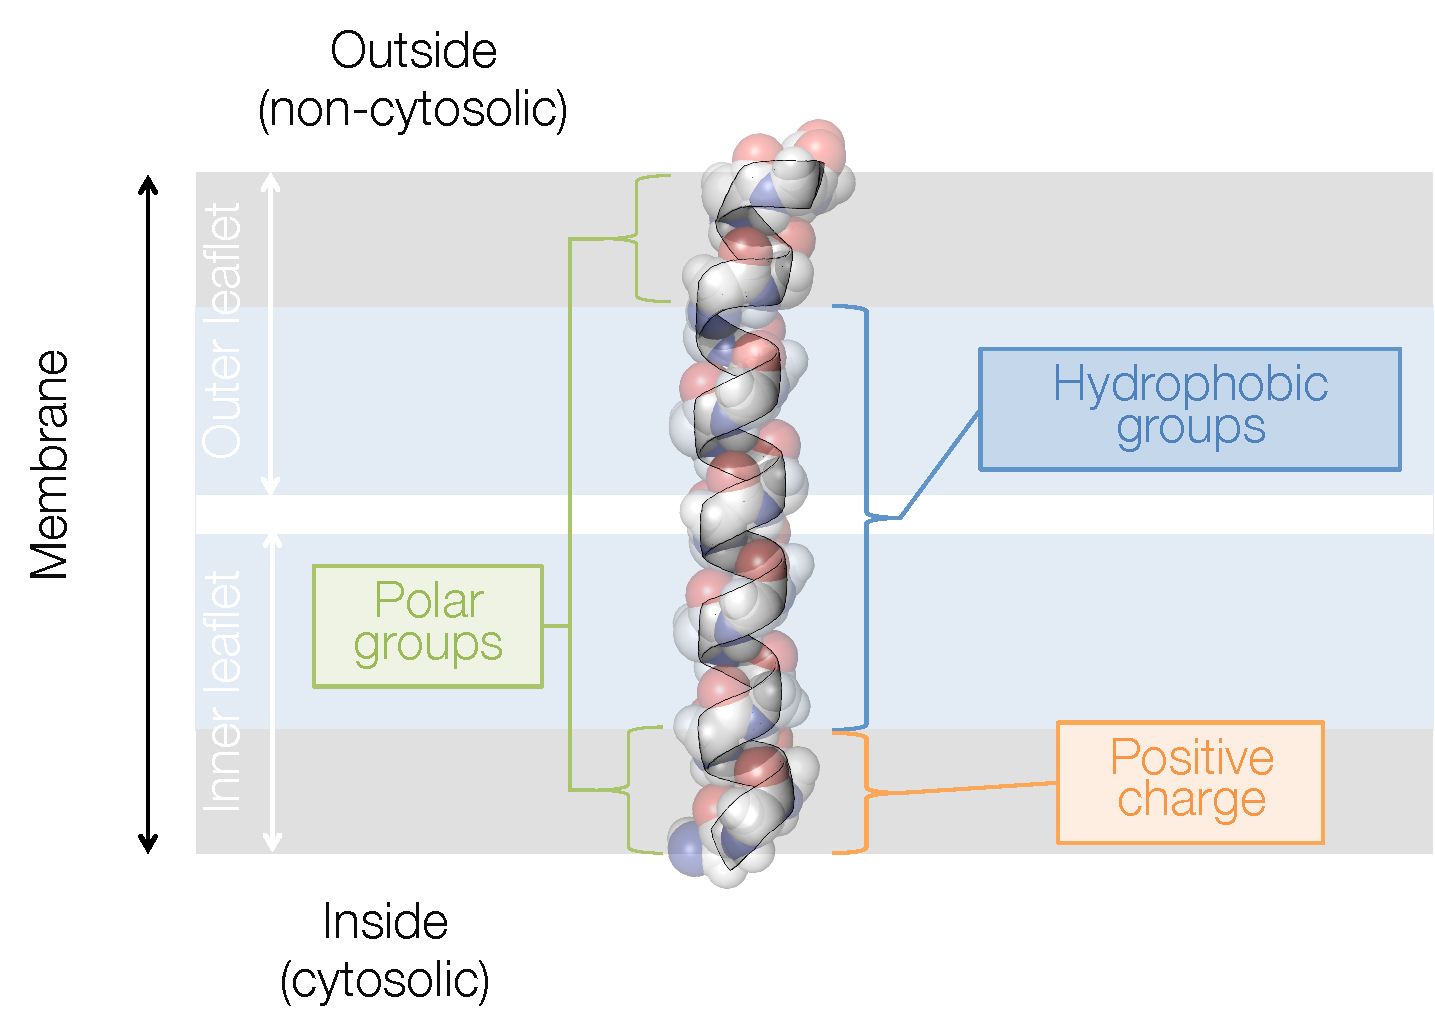
\includegraphics[width=1\textwidth]{Intro/Helix_anatomy}
		\captionof{figure}[A cartoon showing the general components of the membrane and a typical transmembrane helix.]{\textbf{A cartoon showing the general components of the membrane and a typical transmembrane helix}.
		The example used here for illustrative purposes is the transmembrane region of therein (\gls{pdb} 2LK9)~\cite{Skasko2012}.
		Dark grey areas denote the area of lipid head groups.
		The residues found in these areas are often described as flanking regions and are often in contact with the aqueous interface of the membrane.
		The helix core is mostly composed of hydrophobic residues.
		Although the regions labelled here generally hold true in terms of the statistical distribution of polar, non-polar, and charged groups, it is by no means absolute laws and many proteins break these ``rules''~\cite{Sharpe2010, Baeza-Delgado2013, Pogozheva2013}.}

\label{fig:helixcartoon1}
\end{figure}

% Figure: A cartoon depicting various problematic, yet biologically observed topologies and lengths that the alpha helices can adopt.
%From left to right: a typical and traditional \gls{tmh}, an exceptionally long \gls{tmh}, a \gls{tmh} that lies flat in the interface region, a kinked helix that enters and exits the bi-layer on the same leaflet, a \gls{tmh} that is not long enough to span the entire membrane.
%These exceptional formations present a challenge for topology predictions of the loop regions.

The language used to describe \gls{tmh}s varies somewhat across the literature, primarily due to a changing understanding of \gls{tmh} general structure and relevance to function over the last 15 years or so.
There is a general composition of a \gls{tmh} despite specific protein and membrane constraints~\cite{Sharpe2010}.

%This paragraph should certainly be changed to the updated one from the manuscript.
A study by Baeza\---Delgado \textit{ et al.} from 2013~\cite{Baeza-Delgado2013} looked at \gls{tmh}s with known topology and structure in 170 integral membrane proteins from a manually maintained database of experimentally confirmed \gls{tmp}s; MPTopo~\cite{Jayasinghe2001}.
The group examined the distribution of residues along the \gls{tmh}s.
As expected, half of the natural amino acids are equally distributed along transmembrane \gls{tmh}s whereas aromatic, polar, and charged amino acids along with proline are biasedly near the flanks of the \gls{tmh}s~\cite{Baeza-Delgado2013}.
It has been noted that transitions between the polar and non-polar groups at the ends of the hydrophobic core occur in a more defined edge on the cytoplasmic side than at the extracytoplasmic face when counting from the middle of the helix outwards~\cite{Baeza-Delgado2013}.
This is probably reflecting the different lipid composition of both leaflets of biological membranes~\cite{Baeza-Delgado2013}.

A previous study by Sharpe \textit{et al.} from 2010 used 1192 human and 1119 yeast predicted \gls{tmh}s that were not structurally validated to further explore the difference in \gls{tmh} and leaflet structure by exploiting the evolutionarily conserved sequence differences between the \gls{tmh} in the inner and outer leaflets~\cite{Sharpe2010}.
%\gls{tmh}s from vertebrates and invertebrates were found to be reasonably similar compositionally.
The differences in consensus \gls{tmh} structure implies that there are general differences between the membranes of the Golgi and \gls{er}.
The abundance of serines in the region following the lumenal end of Golgi \gls{tms}s probably reflects the fact that this part of many Golgi enzymes forms a flexible linker that tethers the catalytic domain to the membrane~\cite{Sharpe2010}.

\subsubsection{The ``positive\--inside'' rule}

Two publications by von Heijne coined the ``positive-inside'' rule demonstrated the practical value of positively charged residue sequence clustering in topology prediction of \gls{tmh}s in bacteria~\cite{VonHeijne1989,Andersson1992}.
It was clearly defined and shown that positively charged residues more commonly were found on the ``inside'' of the cytoplasm rather than the periplasm of \textit{ E.
coli}.
More recently still large-scale sequence analysis of \gls{tmh}s from different organelle membrane surfaces in eukaryotic proteomes, show the clustering of positive charge being cytosolic~\cite{Sharpe2010, Baeza-Delgado2013, Pogozheva2013}.

\subsubsection{The aromatic belt}

Tyrosine and tryptophan residues commonly are found at the interface boundaries of the \gls{tmh} and this feature is called the ``aromatic belt''~\cite{Hessa2005, Granseth2005, Sharpe2010, Baeza-Delgado2013, Nilsson2005a}.
Not all aromatic residues are not found in the aromatic belt; phenylalanine has no particular preference for this region~\cite{Granseth2005, Braun1999}.
However, it still remains unclear if this is to do with anchoring or translocon recognition~\cite{Baeza-Delgado2013}.

A study of conserved tryptophan residues during folding of integrin $\alpha$II$\beta$3 \gls{tm} complex demonstrated the anchoring effects of tryptophan (0.4 kcal/mol contribution to membrane stability) in \gls{tmh}s is greater than the other residues~\cite{Situ2018}. It was suggested that the wide amphiphilic range (the stabilising energetic contribution in either hydrophobic or polar sites) of tryptophan complements the heterogeneity and asymmetry of mammalian membrane lipids in particular.

The tyrosine side chain is a 6\--carbon aromatic ring with an OH group attached.
Tryptophan has two aromatic rings that contribute to a large hydrophobic ring-structure.
Phenylalanine, although aromatic, is hydrophobic, and unlike tyrosine and tryptophan is typically found in the transmembrane part rather than the interfacial parts of \gls{tmh}s.
The aromatic rings of tryptophan and tyrosine are buried close to, or within, the hydrophobic core, while the hydrophilic portion can interact with the polar lipid head\--groups at the interface between the lipids and the water environment.
Other factors such as the aromaticity, size, rigidity and shape of tryptophan, rather than its dipolar character, has also been suggested as the primary reasons for its interfacial preference and indeed interfacial localisation preference could be the result of a combination of all of these factors \cite{Yau1998}.


\subsubsection{Snorkelling}

Broadly speaking, \gls{tmh}s are non-polar.
However, some contain polar and charged residues in the helix itself.
Whilst this might seem thermodynamically unstable at first glance, a molecular dynamic feature called the ``snorkel'' effect explains in part how this is possible~\cite{Chamberlain2004, Strandberg2003}.
Simply put, the snorkelling effect involves the long flexible side chain of leucine reaching the water interface region to interact with the polar head-groups of the bilayer even when the $\alpha$ helix backbone is pulled into the hydrophobic layer~\cite{Krishnakumar2007}.
This has also been suggested to allow helices to adapt to varying thicknesses of the membrane~\cite{Kandasamy2006}.
More recently it was found that although in simulations the energetic cost of arginine at the centre of the \gls{tmh} is large, \textit{in vivo} experimentation with the Sec61 translocon reveals a much smaller penalty~\cite{Ulmschneider2017}.
That same study also found that in \gls{md} simulations, snorkelling, bilayer deformation, and peptide tilting combined to be sufficient to lower the thermodynamic stability penalty of arginine insertion so that hydrophobic \gls{tmh}s with a central arginine residue will readily insert into the membrane.


\subsection{The hydrophobicity of transmembrane segments}\label{section:hydrophobicityscales}

Perhaps the most prevalent and important feature of the transmembrane regions is the membrane\--spanning region which is composed mostly of non-polar residues.
The importance of hydrophobicity on the effectiveness of membrane anchoring has been known for some time~\cite{Davis1985}.
More recently the hydrophobic group region has been associated with cell localisation and a broad range of biochemical functions~\cite{Junne2010, Sharpe2010, Wong2012}.

Over the last 50 years or so, there have been many attempts to use hydrophobicity scales of residues to predict structural classifications of proteins.
Due to the vast amounts of scales, major efforts have been made to compare them to identify which ones are better for which tasks of identifying structural elements~\cite{Simm2016, Peters2014}.
Simm \textit{ et al.} 2016~\cite{Simm2016} compared 98 scales and found that the accuracy of a scale for secondary structure prediction depends on the spacing of the hydrophobicity values of certain amino acids but generally that the methods behind the scales don't affect the separation capacity between $ \beta $ sheets or $ \alpha $ helices.

Throughout this thesis, several scales are used to evaluate and estimate hydrophobic values of peptide chains.
All the scales aim for quantifying the hydrophobic values of each residue.
There are several key differences in their methodology, assumptions, and aims.
Ultimately, all the scales are attempting to allow estimation of ${\Delta G}_{whf}$; the free energy of a folded helix ($ f $) from the water ($w$) into the membrane core ($h$).
This free energy measurement is regarded as being currently experimentally inaccessible~\cite{Cymer2015}.

Although as a trend most of the scales agree, because of the methodological differences, there are indeed variations of values even after normalisation.
Due to these discrepancies, it is preferable and typical amongst the literature to use several scales to verify the observable trends resulting from interpretation from an individual scale.
Notably, one of the classic scales, Kyte \& Doolittle Hydropathy scale shows a striking similarity to the modern Hessa's ${\Delta G}_{app}^{aa}$ scale, and that generally the ``better'' scales for \gls{tmh} prediction count proline as hydrophilic, and focus on helix recognition rather than amino acid analogues~\cite{Peters2014}.
In $\alpha$ helices from soluble proteins, proline is almost always a helix breaker, and $\alpha$ helix prediction scales don't even attempt to quantify a proline scoring penalty, whereas they are highly tolerated in \gls{tmh}s.
Several of the scales used throughout this thesis are overviewed below.

\subsubsection{Kyte \& Doolittle hydropathy scale}

The Kyte \& Doolittle scale \cite{Kyte1982} is based on the water\---vapour transfer free energy and the interior-exterior distribution of individual amino acids determined previously \cite{Chothia1976}.
The Kyte \& Doolittle gave a composite score to each amino acid based on evidence from previous experiments in the literature, scaling them between -4.5 and +4.5.
These experiments included the molal volumes of model compounds for the side\--chain R groups \cite{Wolfenden1979, Cohn1934, Traube1899}, the water vapour partition coefficients \cite{Hine1975, Wolfenden1979}, and water\--ethanol transfer free energies \cite{Cohn1943, Nozaki1971}.
However, alanine, tyrosine, leucine, and proline scores were subjectively modified.
The authors found it difficult to accept that the single methyl group from alanine would have more hydrophobic force than leucine, which contains 4 methyl groups so the score was arbitrarily lowered to halfway between the originally determined score and the score of glycine.
Tyrosine and leucine had their hydropathy values raised to one closer to the water vapour transfer free energy than experimental data suggested.
In the case of proline, no suitable model existed and it tends to become buried, indicating that it is fairly hydrophilic.
However, because it contains three methyl groups, the score considers it more hydrophobic than the experiments suggested.
The authors stated: ``None of these last 3 adjustments, the result of personal bias and heated discussion between the authors, affects the hydropathy profiles in any significant way''\cite{Kyte1982}.
Arginine represents the bottom of the scale, arbitrarily set at -4.5.

\begin{figure}[ht]
\centering
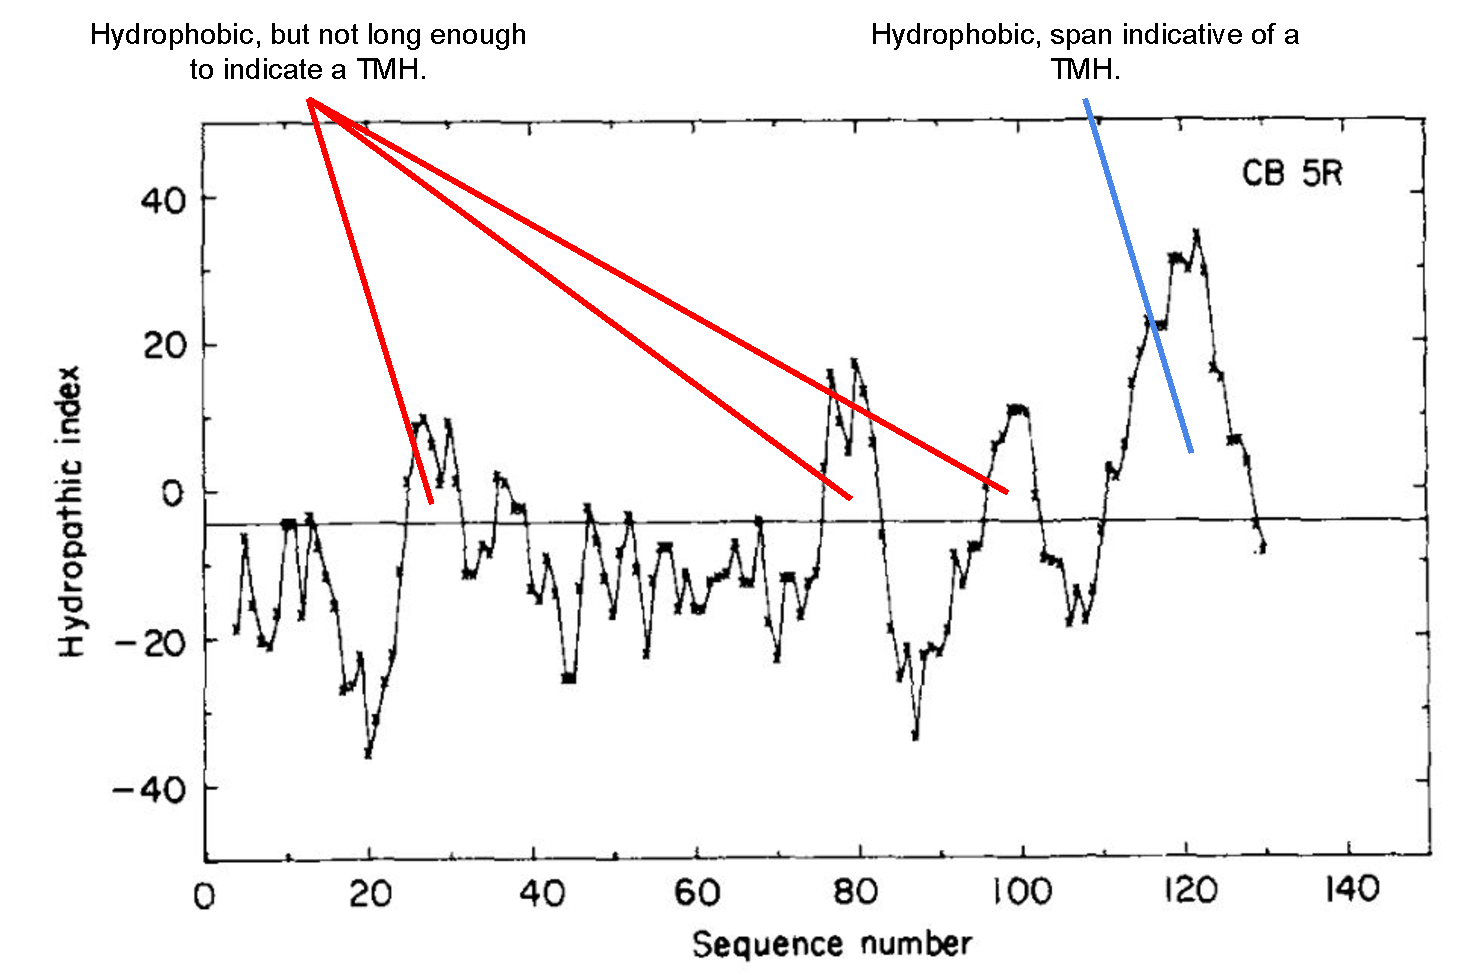
\includegraphics[width=1\textwidth]{Intro/kyte}
		\captionof{figure}[The hydropathic index of rabbit cytochrome b5.]{\textbf{The hydropathic index of rabbit cytochrome b5.}
		The hydropathic index according to the Kyte \& Doolittle scale \cite{Kyte1982} is given on the vertical axis and the sequence number is on the horizontal axis.
		Whilst there are several peaks above 0, only one is sustained for around 20 residues near the c\--terminal.
		Cytochrome b5 is a \gls{ta} protein with an exceptionally polar \gls{tmh} for an anchor \cite{Brambillasca2006}, demonstrating the sensitivity of this method.
		Figure adapted from Kyte \& Doolittle, 1982 \cite{Kyte1982}.
		}
\label{fig:kyte}
\end{figure}

An algorithm called SOAP was used to scan a window of $\pm$10 residues either side of each residue (allowing for half windows) across a protein to take the mean average of each position and plot them on a profile (Figure \ref{fig:kyte}).
Sustained areas of high hydrophobicity were indicative of a \gls{tmh}~\cite{Kyte1982}.

\subsubsection{Hessa's biological hydrophobicity scale}
This is arguably the most biologically relevant scale~\cite{Peters2014} and is often called the ${\Delta G}_{app}^{aa}$ scale.
The scale is based on an experimental method where the free energy exchange during recognition of designed poly-peptide \gls{tmh} by the \gls{er} Sec61 translocon occurred~\cite{Hessa2005}.
These measurements were then used to calculate a “biological hydrophobicity scale.” The original study reported positional variance in some residues and is strictly valid only for residues in the core of the \gls{tmh}.
A more refined study quantified the positional dependencies of each amino acid type~\cite{Hessa2007}.

\subsubsection{White and Wimley octanol \--- interface whole residue scale}
This scale is calculated from two other scales; the octanol scale, and the interface scale~\cite{White1999}.
This scale is fundamentally based on the partitioning of host-guest pentapeptides (acetyl-WL-X-LL-OH) and another set of peptides (AcWLm) between water and octanol, as well as water to \gls{popc}.

\subsubsection{The Eisenberg hydrophobic moment consensus scale}
The Eisenberg scale is a consensus scale based on the earlier scales from Tanford~\cite{Nozaki1971}, Wolfenden~\cite{Rose1993}, Chothia~\cite{Chothia1976}, Janin~\cite{Janin1979},  Wolfenden~\cite{Wolfenden1981}, and the von Heijne scale~\cite{VonHeijne1979}.
The scales are normalised according to serine~\cite{Eisenberg1984}.
The automatic TRANSMEM annotation currently used in UniProt is according to TMHMM~\cite{Krogh2001}, Memsat~\cite{Jones2007}, Phobius~\cite{Kall2004} and the hydrophobic moment plot method of Eisenberg and coworkers~\cite{Eisenberg1984}.

\subsection{Sequence complexity}
Whilst identifying \gls{tmh} presence in a protein is somewhat trivial with modern tools, the role it plays within the membrane is hard to determine. Sequence properties that can be analysed by bioinformatics, the sequence information complexity and hydrophobicity, of the \gls{tmh} have been used to predict the role of the \gls{tmh} as either functional or structural, and as a discrete cluster from other SCOP annotated helices~\cite{Wong2012}.
Those findings demonstrated that the sequence of the \gls{tmh} holds valuable information regarding biological roles, and forms the basis of our interest in the link between the polarity of a helix and functional activity beyond structural anchoring.

TMSOC's z-score is able to distinguish between functionally active~\gls{tmh}s and those only associated with anchoring~\cite{Wong2011, Wong2012}.
This was determined with the annotation of \gls{tmh}s from the UniProt database (303 membrane anchors and 1741 functional TM helices) from UniProt \cite{TheUniProtConsortium2014} and tested with 181132 \gls{tmh} sequences.
Two peaks can be observed when stratifying the hydrophobicity and the sequence complexity of the \gls{tmh}s (Figure \ref{fig:complexity}).
These peaks correspond with the ``simple'' and ``complex'' \gls{tmh} annotation.

\begin{figure}[ht]
\centering
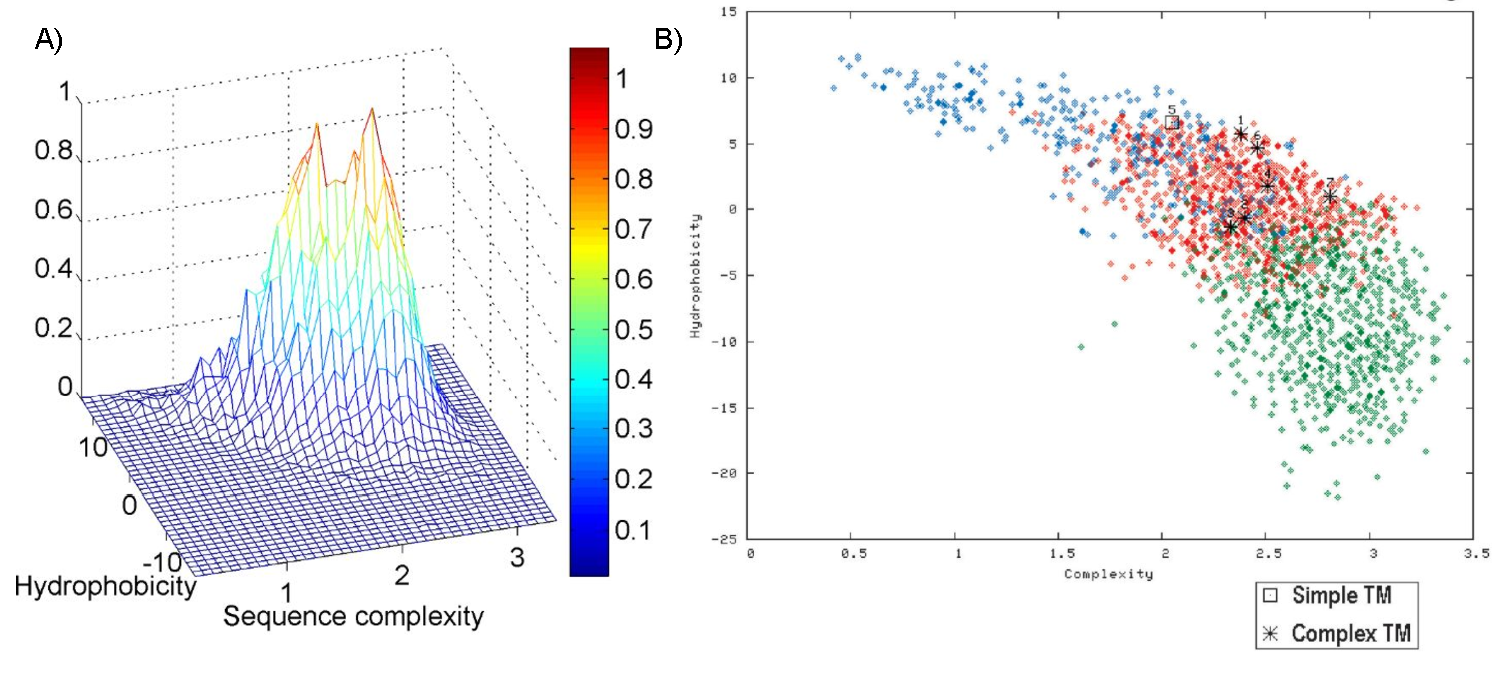
\includegraphics[width=1\textwidth]{Intro/complexity}
		\captionof{figure}[The hydrophobic\--complexity continuum distinguishes between transmembrane helix anchors and those with function beyond anchoring.]{\textbf{The hydrophobic\--complexity continuum distinguishes between transmembrane helix anchors and those with function beyond anchoring.}
		A) Two distinct points can be observed when plotting sequence complexity on the x\--axis, frequency on the y\--axis, and hydrophobicity on the z\--axis of \gls{tmh}s from UniProt.
		These peaks were shown to correspond to the membrane anchor and functional \gls{tmh} populations.
		From Wong \textit{et al.,} 2011 \cite{Wong2011}.
		B) The $\protect\alpha$ helix hydrophobicity complexity continuum stratified by hydrophobicity (vertical axis) and complexity (horizontal axis).
		In blue are the membrane anchors, in red are the \gls{tmh} with function, and in green are non\--\gls{tm} $\protect\alpha$\--helices from SCOP \cite{Murzin1995}.
		Clear distinctions can be made between the 3 groups and in fact, a composite z-score of the distance of these two factors from the functional \gls{tmh} group allows prediction of which group a \gls{tmh} belongs to \cite{Wong2011, Wong2012}.
		From Wong \textit{et al.,} 2012 \cite{Wong2012}.
		}
\label{fig:complexity}
\end{figure}

The z-score is a product of both hydrophobicity and a Shannon like sequence entropy \cite{Wong2011, Wong2012} of the character string in the~\gls{tmh}. This term is described below in equation~\ref{equation:zscoreterm}.

\begin{equation} \label{equation:zscoreterm}
z({x}_{\Phi},{x}_{c})={(-1)}^{s}\left[\frac{{({x}_{\Phi}-{\mu}_{\Phi})}^{2}}{{\sigma}_{\phi}^{2}}+\frac{{({x}_{c}-{\mu}_{c})}^{2}}{{\sigma}_{c}^{2}}\right]
\end{equation}

Where $x_c$ and $x_\Phi$ are moving window averages of c, the sequence entropy~\cite{Wootton1996}. $\Phi$ is the White and Wimley hydrophobicity~\cite{White1999} for a given segment and $\mu$ and $\sigma$ are the mean and standard deviation of the sequence entropy and hydrophobicity of the functional~\gls{tmh} set, that is those~\gls{tmh}s containing active residues.

Sequence entropy is essentially an estimate of the linguistic entropy of a string.
In the context of biology can be thought of as an estimation of the non-randomness of a sequence.
Sequence complexity can be used to analyse DNA sequences~\cite{Pinho2013, Oliver1993, Troyanskaya2002}, however here we will focus on the analysis of the complexity of a sequence in protein sequences.

Broadly speaking, the information theory entropy of a linguistic string can be defined as in equation~\ref{simpleentropy}.

\begin{equation} \label{simpleentropy}
	H(S)=-{\sum_{i=1}^n {p_i\log_s(p_i)}}
\end{equation}

Where H is the entropy of a sequence (S), and $p_i$ is the probability of a character $i$ through each position (n) in S. This allows us to quantify the average relative information density held within a string of information~\cite{Shannon1948}.

%The compositional complexity is measured over sequence windows.
%The total number of sequences can be calculated by dividing a factorial of the length by the product of the compositions, i.e\  $ N = L!/\Pi{n}_i $ possible sequences given an amino acid composition $\{{{n}_{i}}{\}}_{i}={\min{i}},\ldots,{\max{i}}$ with a window length of $L=\Sigma {n}_i $. 
The SEG algorithm~\cite{WOOTTON1994269, Wootton1996} identifies sub-segments of the raw region which have the lowest probability.
The algorithm searches for and concatenates sub-threshold segments for the Shannon entropy-like term in equation~\ref{shannonentropyliketerm}

\begin{equation} \label{shannonentropyliketerm}
{K}_{2}=-\Sigma\frac{n_i}{L}\log\frac{n_i}{L}
\end{equation}

The lowest probability sub-segment can be defined as $ K_1=\log N/L $.
By altering the window lengths, and the thresholds SEG can be optimised to search for subtle compositional deviations, such as coil-coiled regions.


\section{Biogenesis of transmembrane proteins}
%Depth of secretion pathway (talk about translocons in depth here) & outline post-translational insertion
\subsection{An overview of translocation}
%There are, broadly speaking, 3 types of translocation; BiP-mediated eukaryotic post-translational translocation, bacterial post-translational insertion using the Tat system for folded proteins and the Sec system for unfolded proteins, and co-translational insertion in bacteria through the~\gls{htl} protein complex or its individual components.
In this thesis we focus on co\--translation via the Sec pathway, and on the post\--translational pathway of \gls{ta} proteins in eukaryotic systems (Figure \ref{fig:post-versus-co-translation}).

\begin{figure}[ht]
\centering
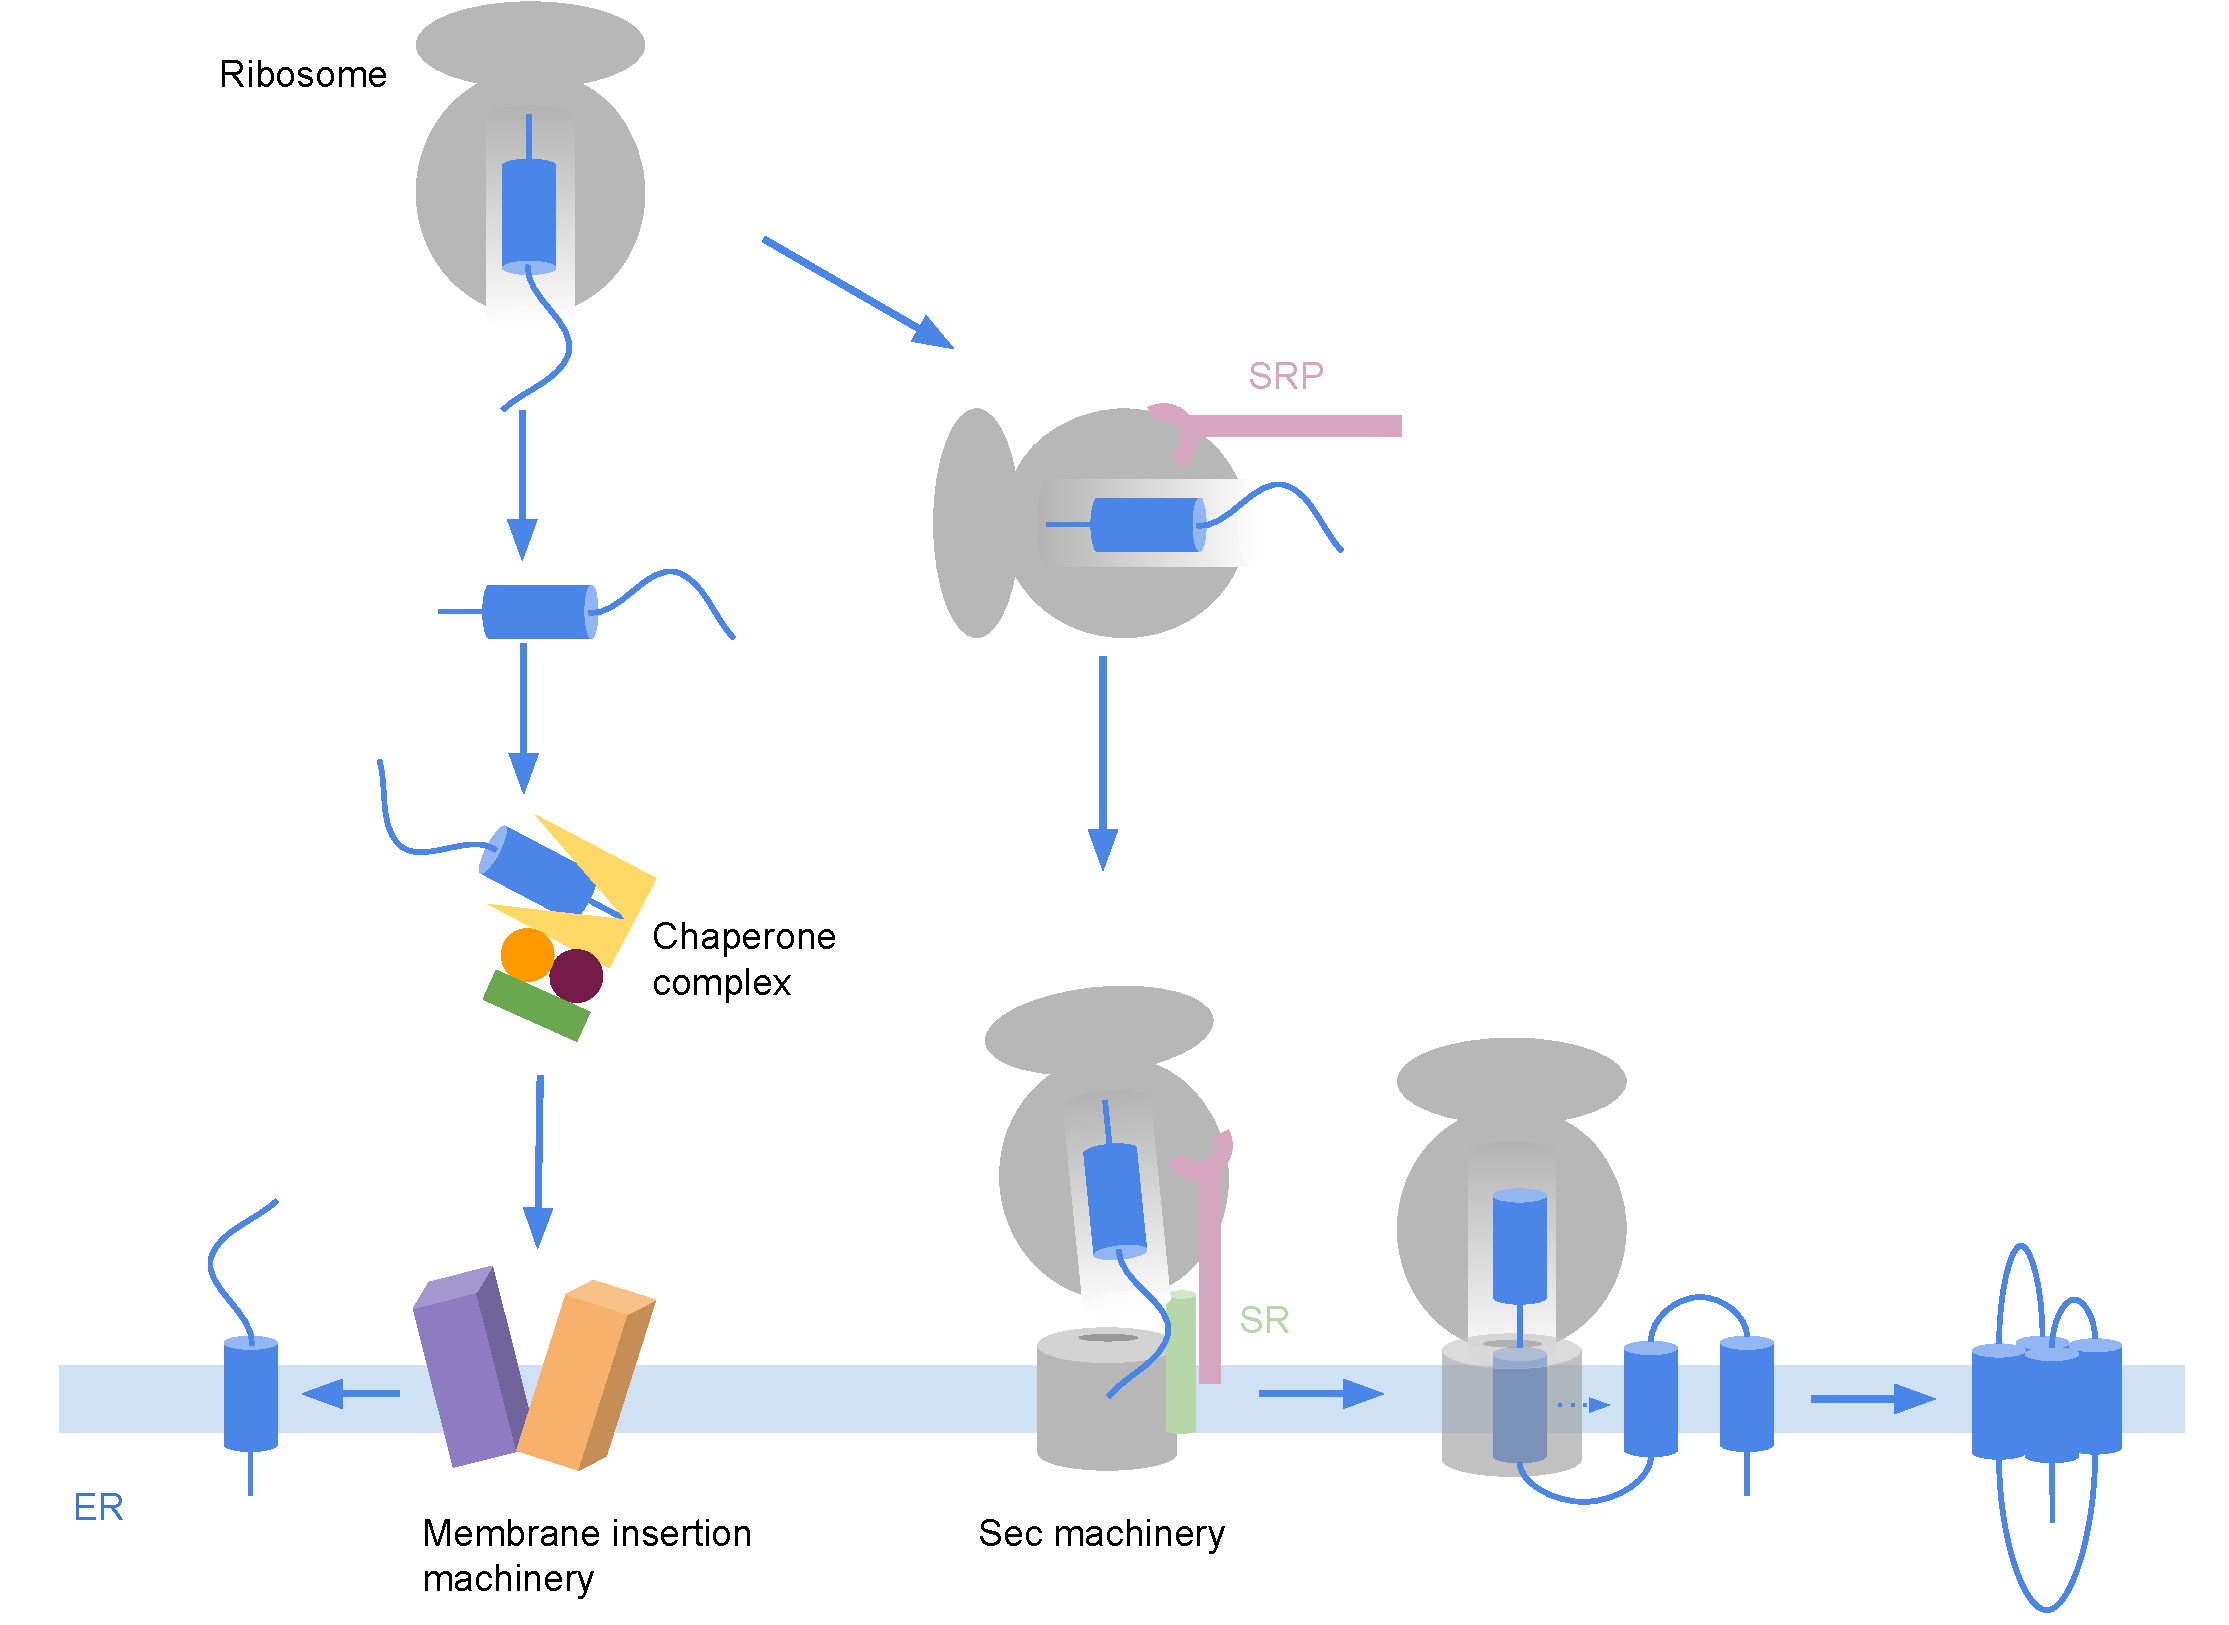
\includegraphics[width=1\textwidth]{Intro/post-versus-co-translation}
		\captionof{figure}[A simplified schematic of the co\--translational Sec pathway and the post\--translational pathway.]{\textbf{A simplified schematic of the co\--translational Sec pathway and the post\--translational pathway.}
		The ribosome translates \gls{rna} to a nascent polypeptide chain.
		In the case of post\--translational insertion (the left\--path), the nascent peptide is released, albeit briefly, to the cytosol.
		Chaperones of various types then shield the protein \gls{tmh} and bring it into contact with various \gls{tm} bound translocation machinery.
		In the case of co\--translation (the right path), the \gls{srp} binds to the emerging signal sequence of the nascent peptide, which slows protein synthesis of the ribosome.
		\gls{srp} then targets the ribosome protein complex to the \gls{sr}, which then moves into contact with the translocon.
		As the nascent protein is inserted into the translocon, \gls{sr} and \gls{srp} detach from the complex and translocation begins.
		}
\label{fig:post-versus-co-translation}
\end{figure}

The Sec pathway is conserved across all life~\cite{Cao2003} and is facilitated by the heterotrimeric SecYEG (prokaryotic) and Sec61 (eukaryotic) translocons.
SecYEG targets proteins to the \gls{pm} (inner membrane) of bacteria.
In bacteria, nearly all \gls{tmp}s are inserted by either the Sec pathway via  SecYEG machinery, or by the structurally unrelated the 5\--fold more abundant YidC machinery \cite{Drew2003, Dalbey2014}, and proteins can often use either pathway.
Sec61 targets proteins to the \gls{er} of eukaryotic cells.
Broadly speaking, these proteins translocate hydrophilic peptides across a membrane whilst also integrating sufficiently hydrophobic sequences to the membrane~\cite{Junne2010, Park2012, Shao2011, Cymer2015}.
In bacteria, the SecY protein is partly encircled by SecE (Sec61$\gamma$ in eukaryotes) which enhances it's stability in the membrane \cite{Kihara1995}.
SecG is made up of two \gls{tmh}s and a cytosolic loop.
It has been associated with SecA dependent translocation of secretory proteins \cite{Duong1997, Koch2000}.
SecA is an ATPase and a membrane channel that can clamp translocating substrates above the SecY pore \cite{Zimmer2008}.

\begin{figure}[ht!]
\centering
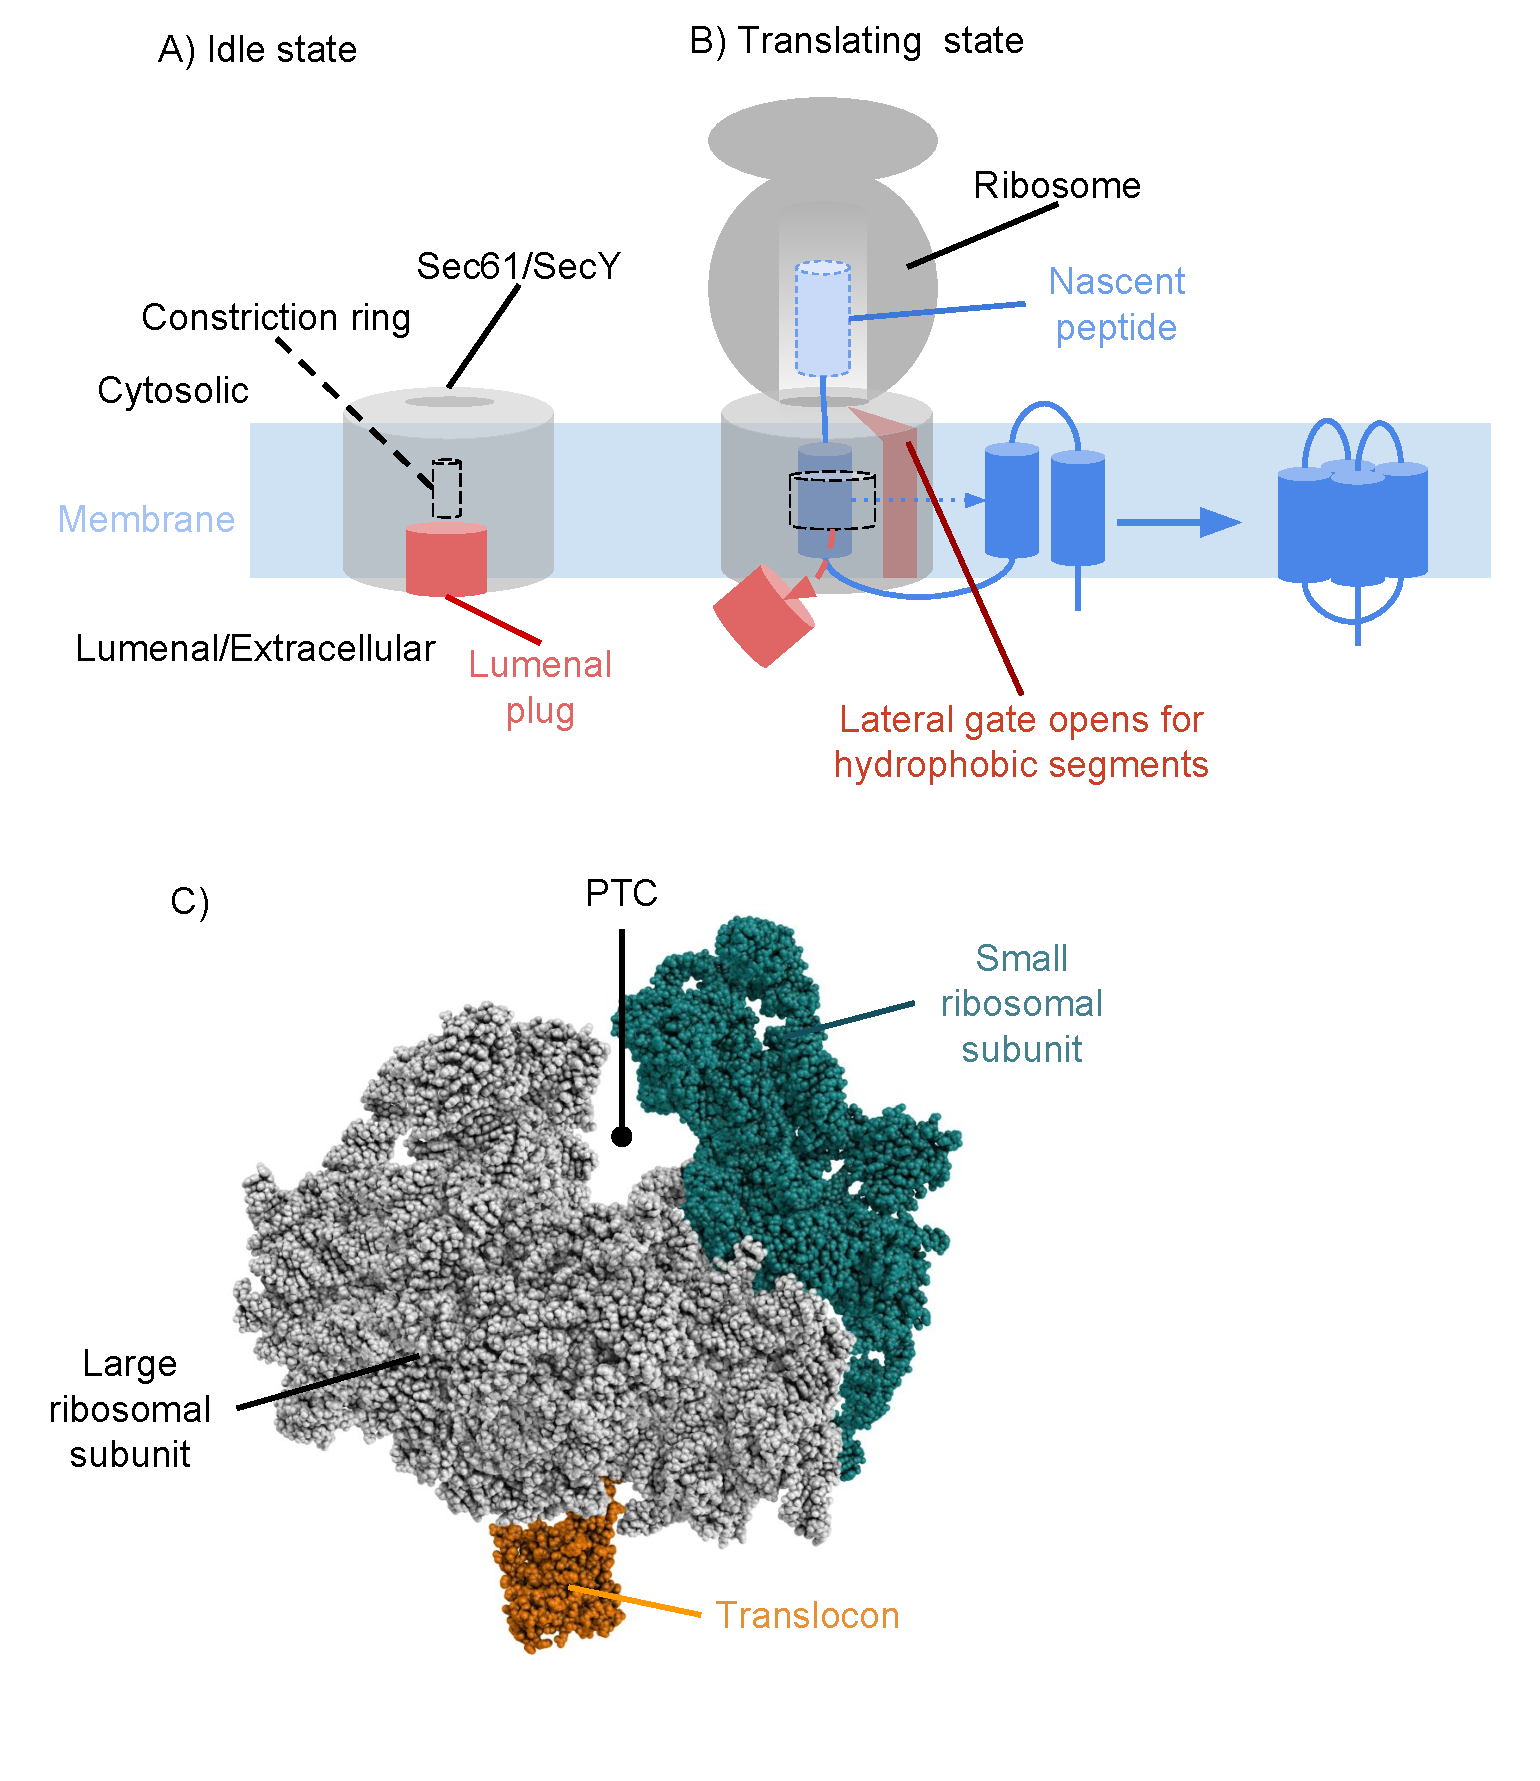
\includegraphics[width=1\textwidth]{Intro/Translocon}
	 \captionof{figure}[The pore, the plug, and the lateral gate of the translocon.]{\textbf{The pore, the plug, and the lateral gate of the translocon.}
	 A) The idle state of the translocon.
	 The pore constriction ring is shown by a dashed transparent cylinder.
	 The plug is in red and the translocon (SecY or Sec61) is in grey.
	 B) The translocating state of the translocon coloured similarly to A, but the plug has moved to allow translocation through the channel, the constriction ring has widened, and the lateral gate opens to allow hydrophobic \gls{tmh}s into the membrane environment.
	 C) A sphere representation of the translocon-ribosome complex structure during translocation.
	 Highlighted are the Sec61 translocon (orange) the ribosome made up of the large 60s subunit and the small 40S subunit and the peptidyl transferase centre (denoted by PTC), the site of translation (PDB 3J7R \cite{Voorhees2014}).
	 Part C redrawn from Voorhees \textit{et al.,} 2014 \cite{Voorhees2014}.

	 }
\label{fig:Translocon}
\end{figure}

Whilst ultimately the translocon machinery is built of multiple subunits, the \gls{tm} translocating protein itself is a 10 \gls{tmh} protein with an hourglass\--shaped interior pore~\cite{Berg2004} (SecY in prokaryotes or Sec61$\alpha$ in eukaryotes).
When translocation is not occurring and the protein is idle, the hydrophobic core is constricted~\cite{Junne2010} and a lumenal plug is in place over the pore resulting in a seal across the \gls{tmp} pore~\cite{Tam2005, Junne2006} that protects the membrane from ion flow \cite{Park2011} (Figure \ref{fig:Translocon}).
\gls{sp}s in stalled nascent chains crosslinked to the lipid and to the translocon machinery \cite{Martoglio1995}, showing that there may be a holding space which exposes the \gls{tmh} to the membrane  interfacial environment before insertion is complete and this was verified by more recent \gls{em} structural study \cite{Gogala2014, Park2012}.

During translocation the plug exits the pore, the constriction ring is opened, and a lateral gate opens between TMH2 and TMH3, and TMH7 and TMH8 to integrate \gls{tmh}s to the membrane~\cite{Berg2004, Petriman2018, Hizlan2012, Bischoff2014, Gogala2014, Egea2010} (Figure \ref{fig:Translocon}).
Mutation experiments on these three features (the plug, constriction ring, and lateral gate) destabilised the closed state of the translocon and resulted in a protein localisation phenotype that suppressed inactivating mutations in signal sequences~\cite{Emr1981, Veenendaal2004, Li2007, Junne2007} and even caused transient channel openings in bacteria~\cite{Saparov2007}.

The \gls{emc} can act as a post\--translational \gls{ta} protein insertase \cite{Guna2018}.
Furthermore, recently it was shown that the \gls{emc} was also able to act cooperatively with the Sec translocon during cotranslational insertion on a subset of multipass \gls{tmp}s in both yeast and human cells \cite{Shurtleff2018}.
Proximity specific ribosome profiling in yeast confirmed that the \gls{emc} engages the translocating multipass \gls{tmp}s, especially those containing charged residues in the \gls{tmh}.
This would explain why it also interacts with \gls{ta} proteins \gls{tmh}s \cite{Guna2018, Shurtleff2018}.
Pulldown experiments revealed that the \gls{emc} stabilised the synthesised \gls{tmp}s and recruited chaperones (both substrate specific and general) that allowed unstable \gls{tmp}s to achieve viable conformations allowing function in the \gls{er} and transport to the Golgi.
In the absence of the \gls{emc}, UPS (a proteasome) degrades the membrane proteins.

This dual function of the \gls{emc} is analogous with YidC \cite{Shurtleff2018} in bacteria which has the role of an insertase \cite{Samuelson2000, Drew2003, Dalbey2014} as well as interacting with SecYEG to stabilise translocated \gls{tmp}s \cite{Nagamori2004}.

\subsection{Signal peptides}
\gls{sp}s are short peptide sequences present at the N-terminus of most secretory pathway destined proteins in both prokaryotes and eukaryotes.
Mutations to the length and composition of the \gls{sp} revealed their composition is essential for effective localised transport, however, they have high compositional variability \cite{VonHeijne1985}.
Like \gls{tmh}s they translocate into the membrane due to their hydrophobic $\alpha$ helix (albeit typically shorter than a \gls{tmh}) and follow the positive\--inside rule.

\begin{figure}[ht]
\centering
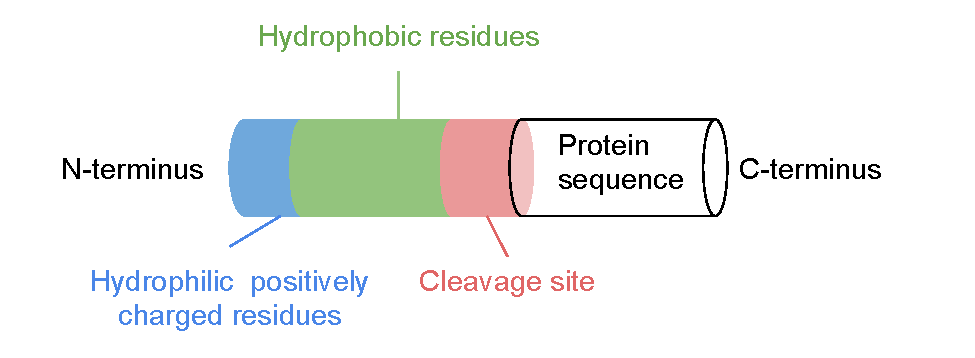
\includegraphics[width=1\textwidth]{Intro/sp}
		\captionof{figure}[The key components of a signal peptide.]{\textbf{The key components of a signal peptide.}
		Signal peptides consist of between 1\--5 hydrophilic charged residues (in blue) at the N terminal, a 7-15 residue hydrophobic region (in green), and a c-region of 3-7 residues that invites cleavage by specific signal peptidase (in red).
	Redrawn from von Heijne, 1990 \cite{VonHeijne1990}.
		}
\label{fig:sp}
\end{figure}


Once the protein is fully translocated and at the correct location within the cell, a three domain signal peptidase cleaves the \gls{sp} from the rest of the protein.
\gls{sp}s can also be experimentally interchanged to proteins from different organisms to target them to cellular locations \cite{Izard1994, Gierasch1989}.

\gls{sp}s are rarely used by \gls{tmp}s with the exception of most type I \gls{tmp}s, which are defined by the presence of an \gls{sp}.
Instead, \gls{tmp}s use their first \gls{tmh} and flanking region as a targeting signal.
Many bioinformatic methods over the last twenty years have aimed to predict \gls{sp}s and sort them from \gls{tmh}s \cite{Choo2009}, however, these methods all struggle to distinguish \gls{sp}s from N-terminal \gls{tmh}s \cite{Petersen2011}.
This is due to the similarities \gls{sp}s have with \gls{tmh}s, and that although \gls{tmh}s are not cleaved, the cleavage site pattern alone cannot effectively separate \gls{sp}s from \gls{tmh}s.
This results in many false positives for \gls{sp} presence in genome\--wide studies \cite{Petersen2011}.
SignalP 4, a neural network based approach, is less effective at predicting cleavage sites or \gls{sp} prediction in the absence of \gls{tmp}s from the dataset, however currently is the most accurate method to distinguish the currently vague differences between \gls{tmh}s and \gls{sp}s \cite{Petersen2011}.

\subsection{$\protect\beta$ sheets in the membrane}

The membrane is critical in maintaining the separation of biochemically distinct compartments.
However, there needs to be a flux not only small molecules but also larger complex structures across these membranes in order to facilitate cellular life.
Whilst the focus of this thesis is primarily on \gls{tmh}s it is important to acknowledge that $\beta$ sheets are another secondary structural element capable of spanning the membrane.

\begin{figure}[ht]
\centering
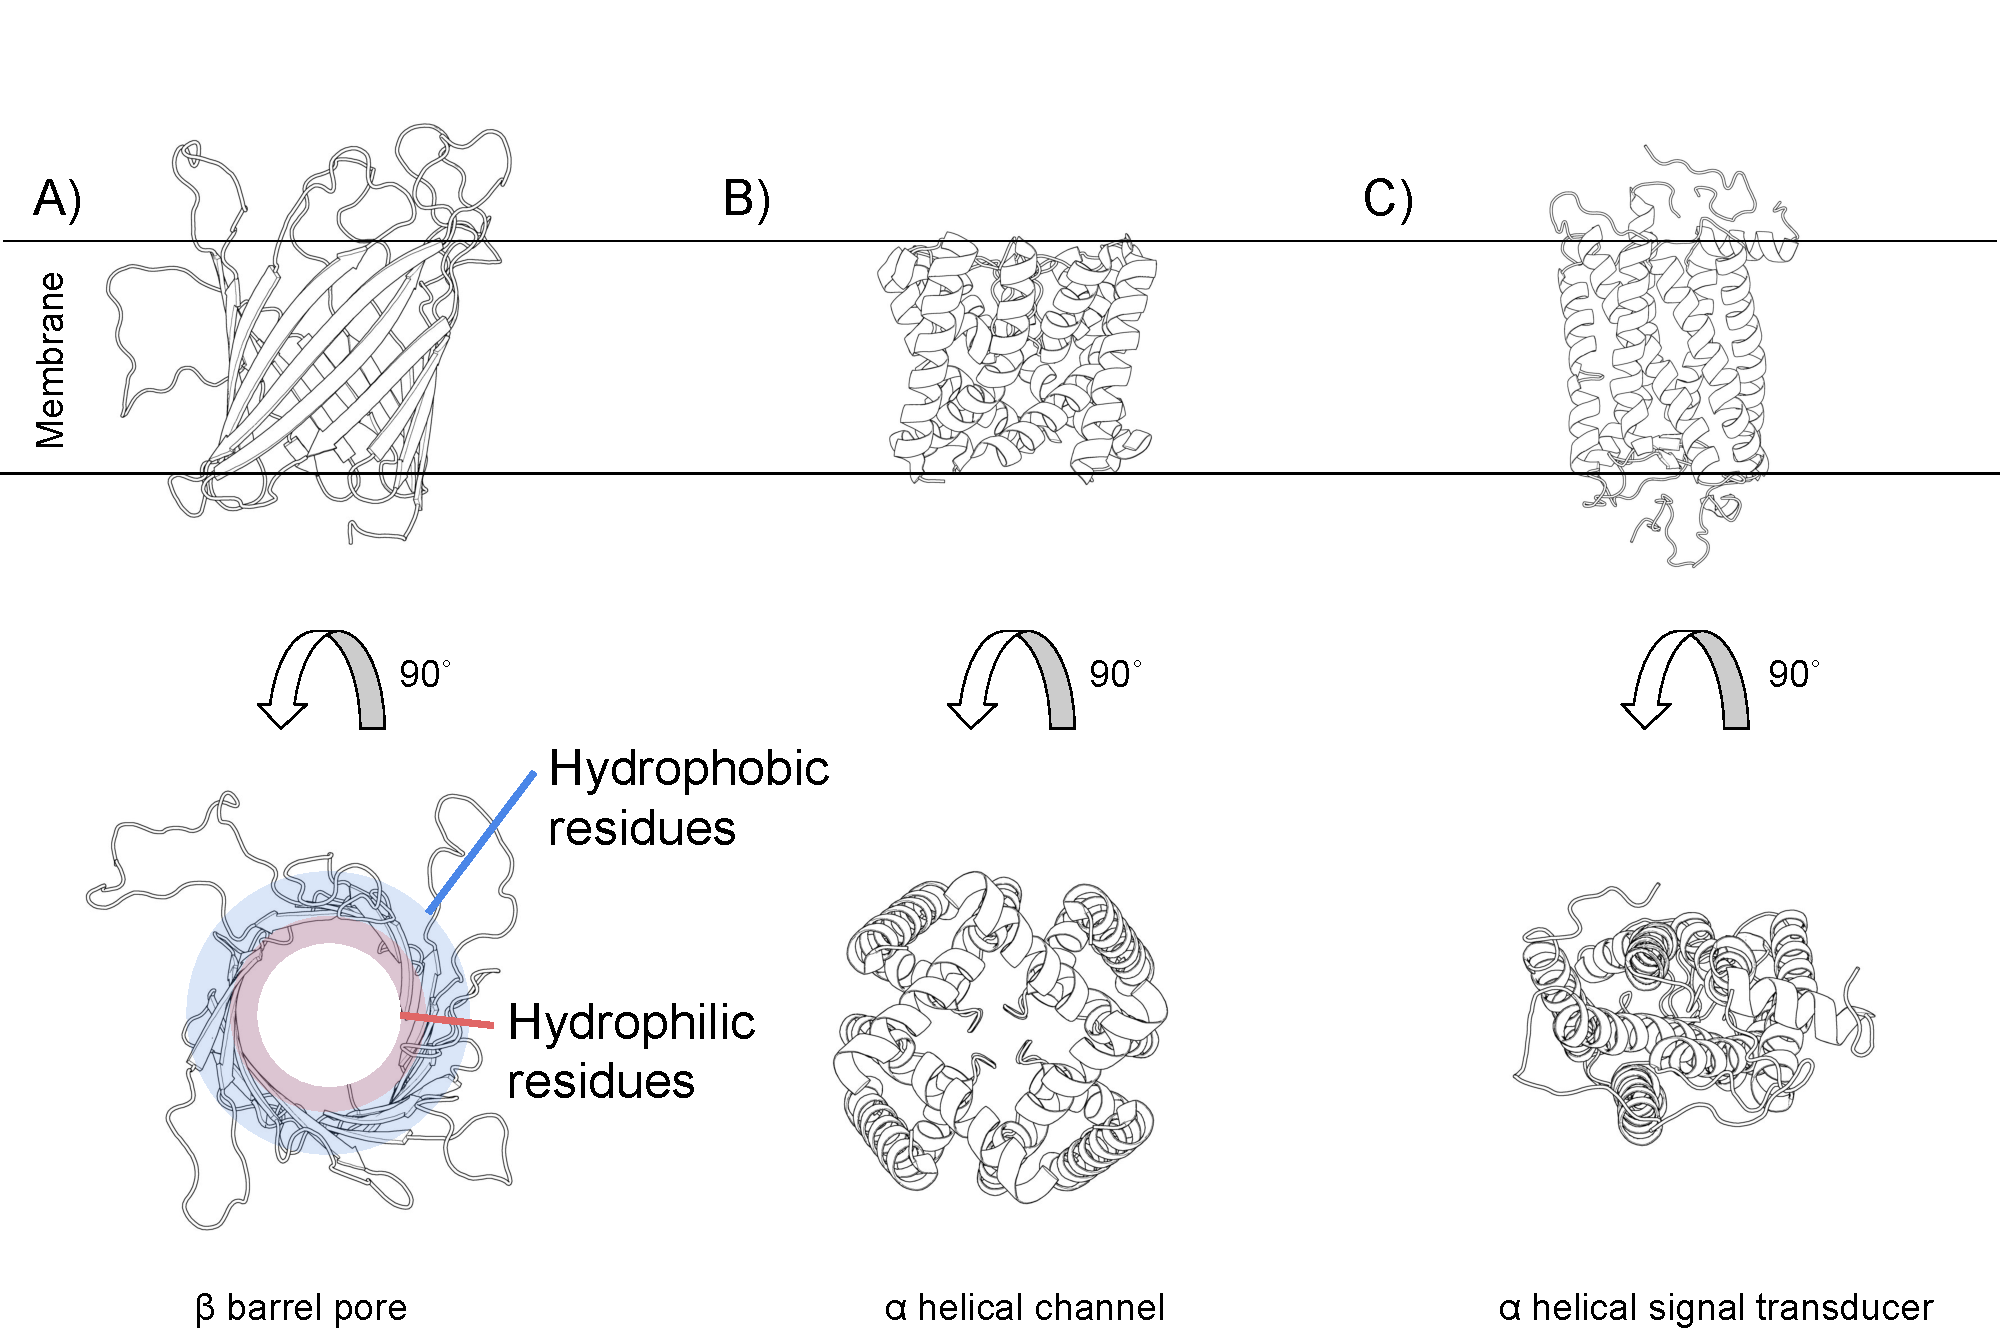
\includegraphics[width=1\textwidth]{Intro/barrel-versus-helix}
		\captionof{figure}[Cartoons showing the structural differences of the outer membrane $\protect\beta$\--barrel proteins, transmembrane $\protect\alpha$\--helix channels, and transmembrane $\protect\alpha$\--helix signal transducers in the membrane.]{\textbf{Cartoons showing the structural differences of the outer membrane proteins, transmembrane helix channels, and transmembrane helix signal transducers in the membrane.}
		The top row shows the proteins traversing the membrane with the interfacial regions denoted by the black lines.
		A) A porous outer membrane protein using $\protect\beta$\--sheets to form a pore\--forming protein structure.
		PDB code 2JQY \cite{Liang2007}.
		B) A highly selective ion channel made up of membrane\--spanning \gls{tmh}s.
		PDB code 4HYO \cite{Posson2013}.
		C) A 7\--\gls{tmh} \gls{gpcr} that receives a signal on one side of the membrane which causes a conformational change influencing the structural arrangement of the tertiary structure on the opposing side of the membrane.
		PDB code 1F88 \cite{Palczewski2000}.
		Note the pore in the $\protect\beta$ barrel protein not present in either the \gls{tmh} channel or the \gls{tmh} transducer.
		}
\label{fig:barrel-versus-helix}
\end{figure}

$\beta$ barrel proteins are present only in a few membrane types; the outer membrane of Gram\--negative bacteria for which they constitute between 2-3\% of the genome \cite{Wimley2003}, and in the outer membranes of eukaryotic chloroplasts and the \gls{mom}.
Their restriction to these membrane types is the result of ancestral symbiogenesis \cite{McFadden2001, Gray1999, Fischer1994, Zeth2010, Fairman2011, Ulrich2015}.

These outer membrane proteins cause the membranes to be permeable, diminishing membrane potential between the outer and the inner membrane.
Unlike the \gls{tmh}s, $\beta$ barrel proteins are permeable to water and many other small molecules often unspecifically due to their large pore (Figure \ref{fig:barrel-versus-helix}).
Integral $\beta$ barrel proteins consist of between 8 and 26 amphipathic antiparallel $\beta$ strands forming a cylindrical pore.
They are capable of active and passive transport, molecule receptors, enzymatic catalysis, structural formation, and translocon machinery \cite{Wimley2003}.

The biogenesis of $\beta$ barrel membrane proteins also differs from that of \gls{tmh}s, and there are differences between prokaryotic and eukaryotic cells.

In Gram\--negative bacteria, the $\beta$ barrel proteins are translated on cytoplasmic ribosomes (Figure \ref{fig:beta-mito-versus-bacteria}).
An N-terminal \gls{sp} sequence allows the protein to pass through the inner membrane to the outer membrane \cite{Driessen2008, Papanikou2007}.
Instead of cotranslational insertion, SecB transports the nascent polypeptide chain to the Sec translocon on the inner membrane \cite{Bechtluft2010}.
$\beta$\--sheets do not trigger the opening of the lateral gate \cite{Ulrich2015}.
Once in the periplasm, the \gls{sp} is cleaved \cite{Paetzel2014} and chaperones, such as the redundant SurA \cite{Lazar1996, Volokhina2011}, DegQ, and Skp \cite{Volokhina2011}, bind to the protein to prevent premature folding.
Once at the inner surface, the BAM complex assembles and integrates the $\beta$ barrel protein into the membrane \cite{Wu2005, Hagan2010} via a lateral opening of one of the BAM subunits, BamA \cite{Noinaj2014}.

\begin{figure}[ht]
\centering
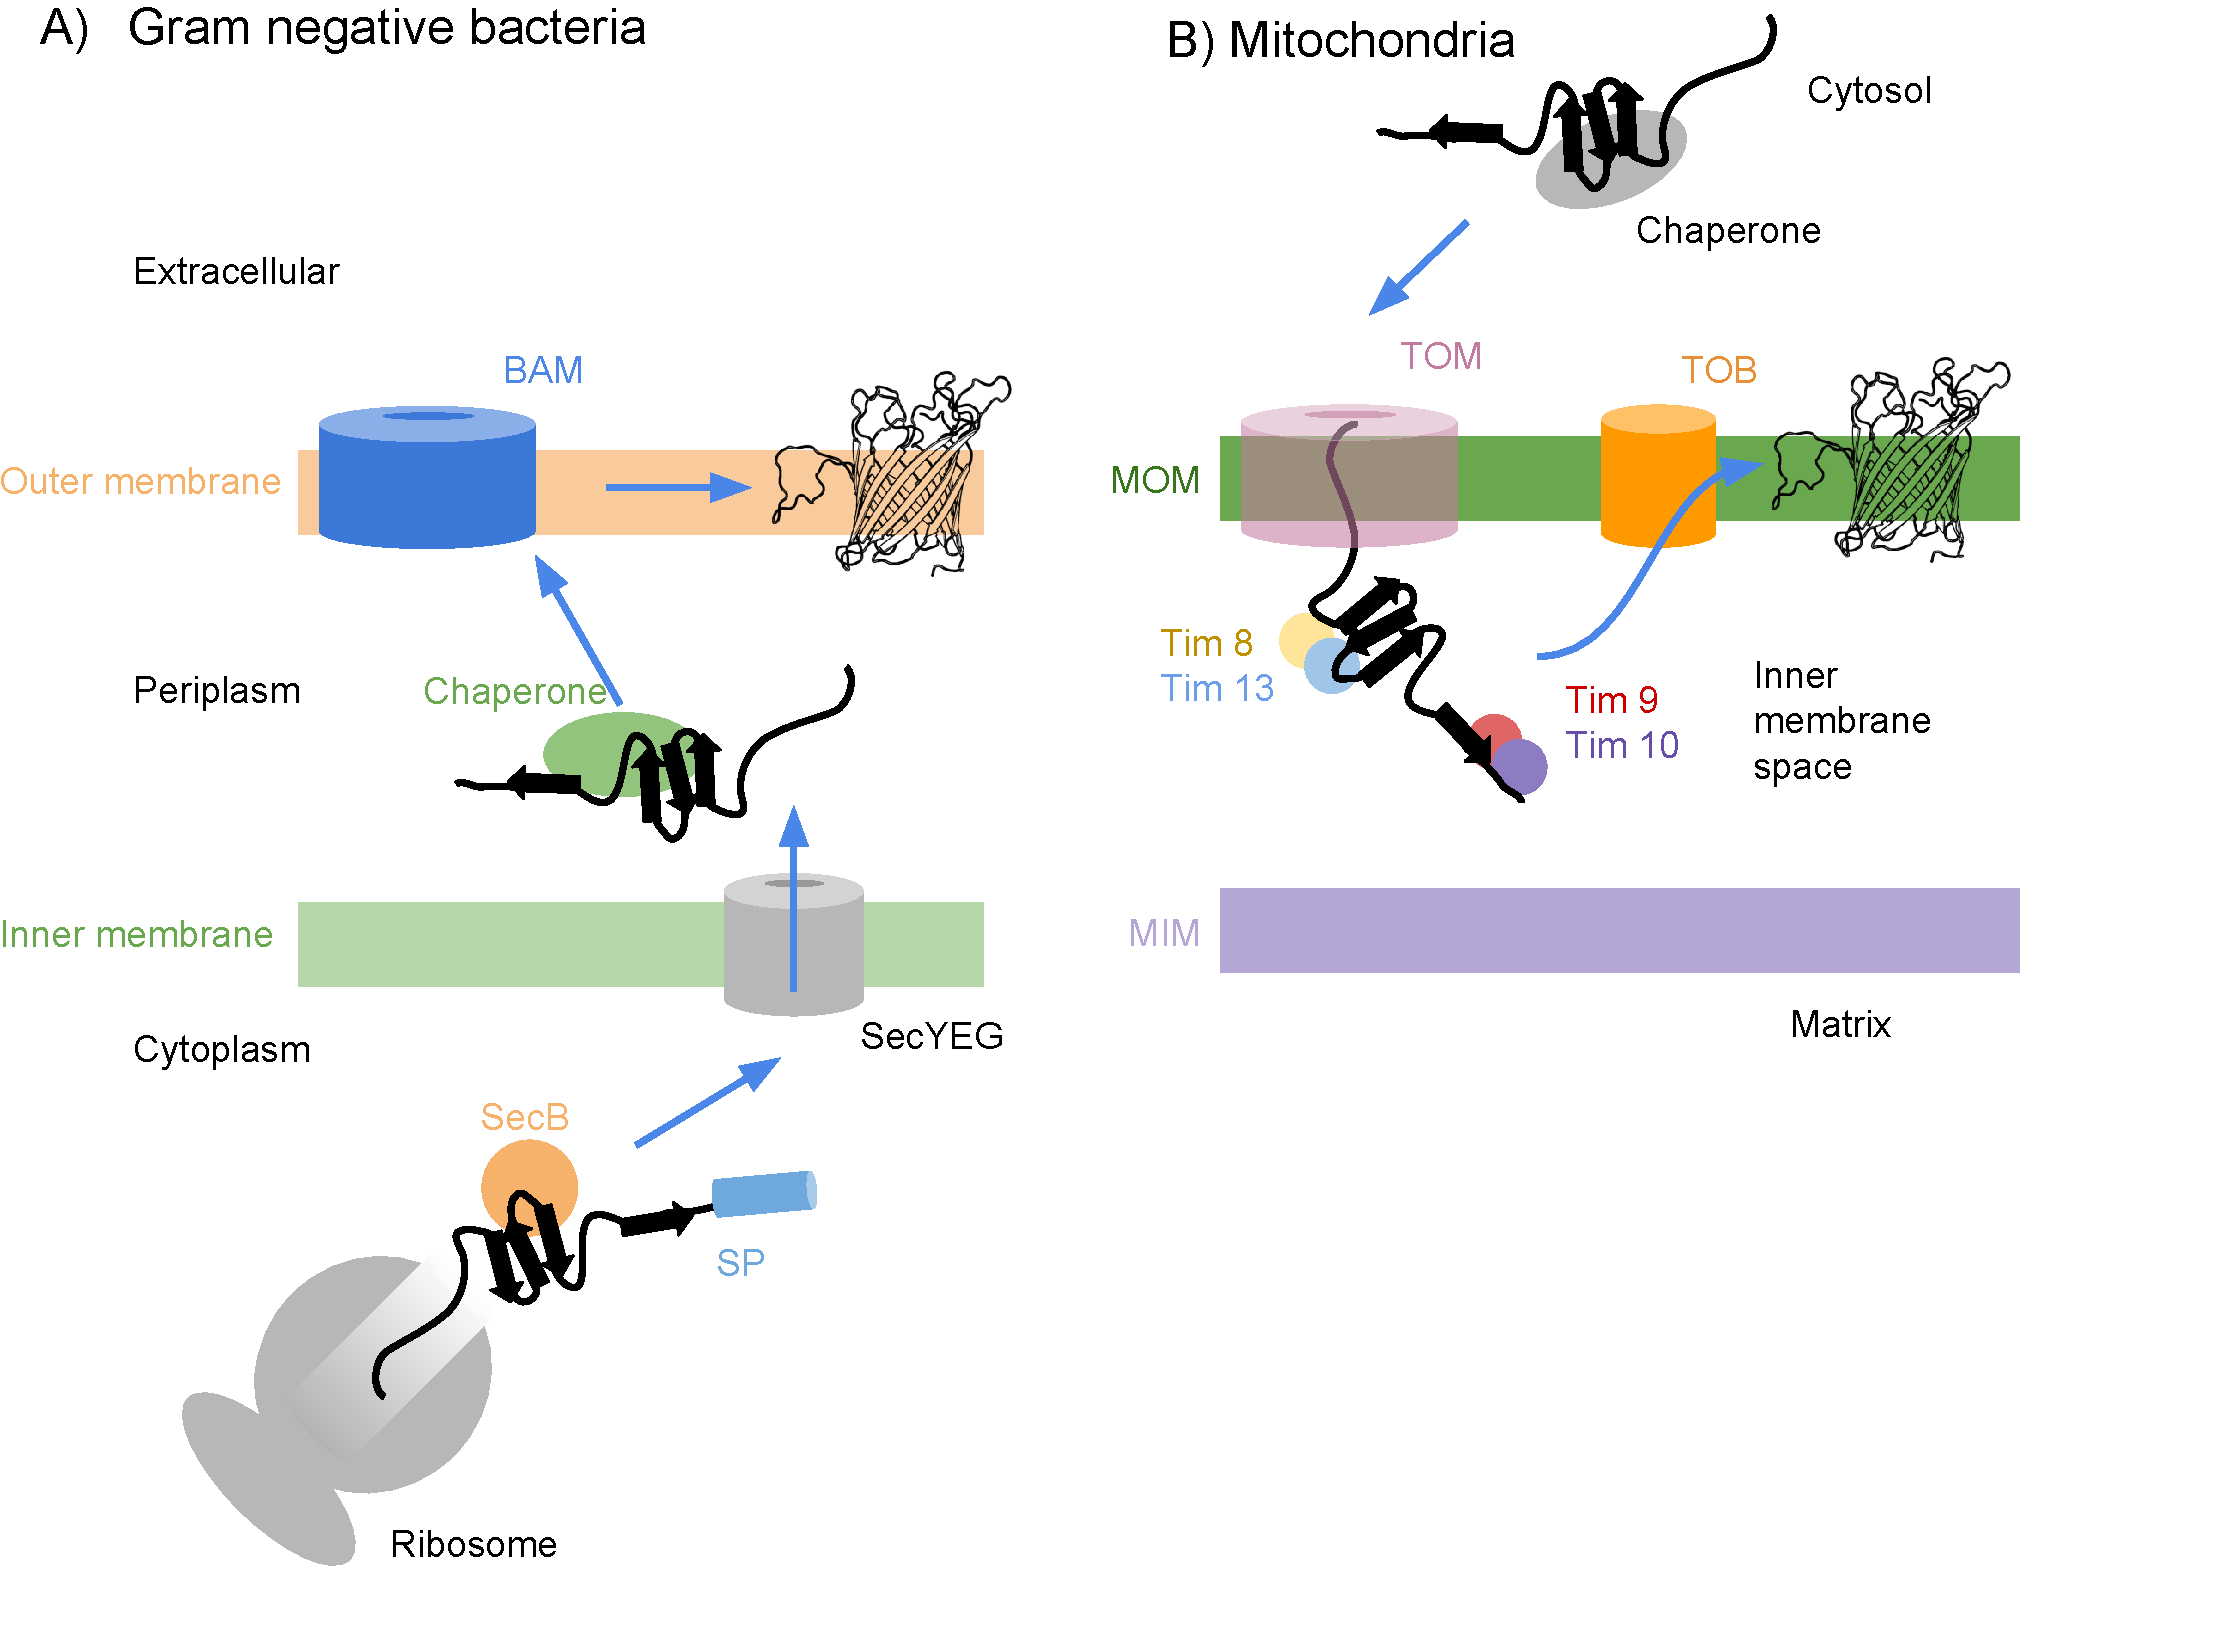
\includegraphics[width=1\textwidth]{Intro/beta-mito-versus-bacteria}
		\captionof{figure}[A cartoon of the biogenesis of $\protect\beta$ barrel membrane proteins in mitochondria and Gram\--negative bacteria.]{\textbf{A cartoon of the biogenesis of $\protect\beta$ barrel membrane proteins in mitochondria and Gram\--negative bacteria.}
		This is an overview of the current model of $\beta$\--barrel protein membrane integration.
		A) In bacteria, SecB chaperones the nascent peptide to SecYEG where it is transported across the inner membrane.
		Once the \gls{sp} is cleaved, the protein is chaperoned to the BAM machinery by SurA, DegQ, or Skp.
		The BAM machinery integrates the protein into the membrane.
		B) After ribosomal translation, the nascent peptide is transported across the \gls{mom} by the \gls{tom} machinery.
		Several Tim recognition molecules then attach to the protein and present it to the TOB insertion machinery, which integrates the protein into the membrane.
		Redrawn from Ulrich \& Rapoport, 2015 \cite{Ulrich2015}.

		}
\label{fig:beta-mito-versus-bacteria}
\end{figure}

Unlike in the bacterial outer membrane, $\beta$-barrel proteins are rare in the mitochondria \cite{Ulrich2015}.
There is Tom40, Tob55, two isoforms of a porin, and Mdm10 \cite{Ulrich2015}.
And yet, indeed it was shown that a $\beta$ barrel protein fragments not found in the eukaryotic proteome called trimeric autotransporter can be recognised and assembled by the mitochondria \cite{Muller2011}.
Since there is no need to cross the inner membrane, mitochondrial proteins do not have the cleavable \gls{sp}, or any other known targeting signal \cite{Ulrich2015}.
After cytosolic ribosomes complete the translation, the $\beta$ barrel proteins are recognised on the mitochondrial surface by the \gls{tom} complex import receptors, handed to the $\beta$ barrel protein Tom40 which is the central machinery for mitochondrial protein import \cite{Chacinska2009}.
After being processed through the \gls{tom} machinery, hexameric chaperone complexes of Tim8 in complex with Tim13, and Tim9 in complex with 10 to the TOB complex (also known as the SAM complex) also on the \gls{mom} which integrates the $\beta$ barrel protein into the membrane \cite{Wiedemann2003, Paschen2003, Gentle2004}.

Whereas mitochondria originated from the ancestral incorporation of $\alpha$\--proteobacteria \cite{Gray1999}, chloroplasts were thought to originate from the incorporation of cyanobacterium \cite{McFadden2001}.
Similarly to mitochondrial $\beta$ barrel proteins, there is no cleavable targeting \gls{sp} targeting for the chloroplast since they integrate on the internal side of the membrane, however much less is known about the precise insertion machinery of $\beta$ barrel proteins at a molecular level in chloroplasts \cite{Ulrich2015}.

Besides the differences in biogenesis between $\beta$ barrel \gls{tmp}s and \gls{tmp}s with \gls{tmh}s as the membrane\--spanning units, there are also biophysical differences.
Membrane\--spanning $\beta$ sheets exhibit a ``positive\--outside'' distribution of positively charged residues \cite{Pogozheva2013}, as opposed to the much more typical positive\--inside distribution \cite{VonHeijne1989, Andersson1992, Pogozheva2013, Sharpe2010, Baeza-Delgado2013}.
Typically, $\beta$ sheets are less hydrophobic than \gls{tmh}s \cite{Tamm2004} as a result of their amphiphilic nature.

\section{The aims of this thesis}

In this thesis, we explore three ideas surrounding the role of \gls{tmh}s in the membrane.

In chapter 2 we explore the sequence composition of large datasets of \gls{tmh}s stratifying them by species, organelle, single\--pass and multi\--pass.
After considering the rarity of certain amino acid types, we show a ``negative\--outside'' tendency in concert with the ``positive\--inside'' rule.
We go on to further divide the single\--pass \gls{tmp}s into complex and simple \gls{tmh}s according to TMSOC.
This reveals that simple \gls{tmh}s have amino acid distribution features along the helix that would optimise for anchoring, however complex \gls{tmh}s are more akin to \gls{tmh}s from multi\--pass \gls{tmp}s.

In chapter 3 we generate an up to date dataset of post\--translationally inserted \gls{ta} proteins based on previous methods and compare the \gls{tmh}s within to a manually curated \gls{ta} protein dataset from UniProt.
This cross\--examination revealed  adaptations in the \gls{tmh} sequences to mitochondrial membranes.
This is likely to play a role in trafficking of the \gls{ta} \gls{tmp} as well as being an adaptation to the differences in the biological composition of the mitochondrial membrane.
% There was as a reversal of the ``positive\--inside'' rule and a reduction in hydrophobicity caused by an abundance of alanine residues in lieu of leucine rather than an increase of polar residues.
We also generate homology models of two spontaneously inserting \gls{tmh}s from \gls{ta} proteins and show that they have an amphipathic surface which may be key to their insertion.

In chapter 4 we look at families of \gls{tmp}s that exhibit a high hydrophobic discrepancy between sequentially adjacent \gls{tmh}s.
The conservation of these pairs across the families corroborates evidence of cooperative \gls{tmh} insertion, showing that marginally hydrophobic \gls{tmh}s could use typical \gls{tmh}s as part of their biogenesis on a larger scale than previously thought.
